\documentclass{scrartcl}

\ifx \GUARDhsrColors \undefined
\def\GUARDhsrColors{}

\usepackage[table]{xcolor}

\definecolor{HSRWhite}{cmyk}{0,0,0,0}

\definecolor{HSRBlue}{cmyk}{1,0.4,0,0.2}
\definecolor{HSRBlue80}{cmyk}{0.8,0.32,0,0.16}
\definecolor{HSRBlue60}{cmyk}{0.6,0.24,0,0.12}
\definecolor{HSRBlue40}{cmyk}{0.4,0.16,0,0.08}
\definecolor{HSRBlue20}{cmyk}{0.2,0.08,0,0.04}

\definecolor{HSRLightGray}{cmyk}{0,0,0,0.30}
\definecolor{HSRLightGray80}{cmyk}{0,0,0,0.24}
\definecolor{HSRLightGray60}{cmyk}{0,0,0,0.18}
\definecolor{HSRLightGray40}{cmyk}{0,0,0,0.12}
\definecolor{HSRLightGray20}{cmyk}{0,0,0,0.06}

\definecolor{HSRSchwarz}{cmyk}{0,0,0,1}
\definecolor{HSRSchwarz80}{cmyk}{0,0,0,0.8}
\definecolor{HSRSchwarz60}{cmyk}{0,0,0,0.6}
\definecolor{HSRSchwarz40}{cmyk}{0,0,0,0.4}
\definecolor{HSRSchwarz20}{cmyk}{0,0,0,0.2}

\definecolor{HSRHematite}{cmyk}{0.6,1,0.4,0.2}
\definecolor{HSRHematite80}{cmyk}{0.48,0.80,0.32,0.16}
\definecolor{HSRHematite60}{cmyk}{0.36,0.60,0.24,0.12}
\definecolor{HSRHematite40}{cmyk}{0.24,0.40,0.16,0.08}
\definecolor{HSRHematite20}{cmyk}{0.12,0.20,0.08,0.04}

\definecolor{HSRLakeGreen}{cmyk}{0.70,0.30,0.45,0.05}
\definecolor{HSRLakeGreen80}{cmyk}{0.56,0.24,0.36,0.03}
\definecolor{HSRLakeGreen60}{cmyk}{0.42,0.18,0.27,0.02}
\definecolor{HSRLakeGreen40}{cmyk}{0.28,0.06,0.13,0.06}
\definecolor{HSRLakeGreen20}{cmyk}{0.14,0.06,0.09,0.01}

\definecolor{HSRReed}{cmyk}{0.10,0.25,0.45,0.60}
\definecolor{HSRReed80}{cmyk}{0.08,0.20,0.36,0.48}
\definecolor{HSRReed60}{cmyk}{0.06,0.15,0.27,0.36}
\definecolor{HSRReed40}{cmyk}{0.04,0.10,0.18,0.24}
\definecolor{HSRReed20}{cmyk}{0.02,0.05,0.09,0.12}

\definecolor{HSRPetrol}{cmyk}{1,0.18,0,0.45}
\definecolor{HSRPetrol80}{cmyk}{0.64,0.08,0.12,0.32}
\definecolor{HSRPetrol60}{cmyk}{0.48,0.06,0.09,0.24}
\definecolor{HSRPetrol40}{cmyk}{0.32,0.04,0.06,0.16}
\definecolor{HSRPetrol20}{cmyk}{0.16,0.02,0.03,0.08}

\definecolor{HSRBasswood}{cmyk}{0.25,0.05,0.70,0.15}
\definecolor{HSRBasswood80}{cmyk}{0.20,0.04,0.56,0.12}
\definecolor{HSRBasswood60}{cmyk}{0.15,0.03,0.42,0.09}
\definecolor{HSRBasswood40}{cmyk}{0.10,0.02,0.28,0.06}
\definecolor{HSRBasswood20}{cmyk}{0.05,0.01,0.14,0.03}


\fi
%%%%%%%%%%%%%%%%%%%%%%%%%%%%%%%%%%%%%%%
%% Makros & anderer Low-Level bastel %%
%%%%%%%%%%%%%%%%%%%%%%%%%%%%%%%%%%%%%%%
\makeatletter
%% Makros für Titel, Autor und Datum
%% Dank diesem Makro stehen Titel, Autor und Datum überall im Dokument zur verfügung
%% Date hat zudem den Default-Wert \today
\def\@Title{}
\def\@Author{}
\def\@Date{\today}
\newcommand{\Title}{\@Title}
\newcommand{\Author}{\@Author}
\newcommand{\Date}{\@Date}
\AtBeginDocument{%
  \let\@Title\@title
  \let\@Author\@author
  \let\@Date\@date
}

%% Makros für den Arraystretch (bei uns meist in Tabellen genutzt, welche Formeln enthalten)
% Default Value
\def\@ArrayStretchDefault{1} % Entspricht der Voreinstellung von Latex

% Setzt einen neuen Wert für den arraystretch
\newcommand{\setArrayStretch}[1]{\renewcommand{\arraystretch}{#1}}

% Setzt den arraystretch zurück auf den default wert
\newcommand{\resetArrayStretch}{\renewcommand{\arraystretch}{\@ArrayStretchDefault}}

% Makro zum setzten des Default arraystretch. Kann nur in der Präambel verwendet werden.
\newcommand{\setDefaultArrayStretch}[1]{%
	\AtBeginDocument{%
		\def\@ArrayStretchDefault{#1}
		\renewcommand{\arraystretch}{#1}
	}
}
\makeatother


%%%%%%%%%%%%%%%%%%%%%%%
%% Wichtige Packages %%
%%%%%%%%%%%%%%%%%%%%%%%
\usepackage[utf8]{inputenc} % UTF-8 unterstützung
\usepackage[english, ngerman]{babel} % Silbentrennung
\usepackage[automark]{scrlayer-scrpage} % Header und Footer
\usepackage{tabularx}
\usepackage{paralist} % Compactitem
\usepackage{tikz}
\usetikzlibrary{positioning,shapes,shadows,arrows}

% Für Abbildungen mit mehreren kleinen Bilder
% Doku: http://www.ctan.org/tex-archive/macros/latex/contrib/caption/
\usepackage{caption}
\usepackage{subcaption}


% Large TODO note
\newcommand{\todo}[1]{%
    \marginpar{\textcolor{red}{ToDo}}%
    \colorbox{red}{\parbox{\linewidth}{\sffamily\textcolor{white}{#1}}}%
    \PackageWarning{ToDo:}{#1!}%
}

\ifx\GUARDmathe\undefined
\def\GUARDmathe{}

\usepackage{amssymb}
% Das mathtools package ist eine Erweiterung zum amsmath package.
% Das amsmath package wird dabei automatisch geladen
\usepackage{mathtools}


% Package mit vielen weiteren Mathe Symbolen
% http://www.ctan.org/tex-archive/fonts/mathabx
\usepackage{mathabx}

\fi
\ifx\GUARDenumitem\undefined
\def\GUARDenumitem{}

\usepackage{enumitem}

\fi

% Seitenränder für Formelsammlungen
\usepackage[left=1cm,right=1cm,top=1cm,bottom=1cm,includeheadfoot]{geometry}

\usepackage{multirow} % Create tabular cells spanning multiple rows
\usepackage{multicol} % In­ter­mix sin­gle and mul­ti­ple columns
\usepackage{rotating} % Rotation tools, including rotated fullpage floats


%%%%%%%%%%%%%%%%%%%%%%%%%%%%%%%%%%%
%% Layout der Kopf und Fusszeile %%
%%%%%%%%%%%%%%%%%%%%%%%%%%%%%%%%%%%
\deftripstyle{zusammenfassung}[0pt][0.5pt]
	{\Title}	% Kopfzeile innen
	{\headmark}	% Kopfzeile mitte
	{\pagemark}	% Kopfzeile aussen
	{\Author}	% Fusszeile innen
	{
\includegraphics[width=1.6cm]{./header/lizenzen/cc-by-nc-sa/small.png}}			% Fusszeile mitte
	{\Date}	% Fusszeile aussen
\pagestyle{zusammenfassung}



% Makros für Verweise auf ein Buch oder Skript
\newcommand{\buch}[1]{$_{\textcolor{HSRLakeGreen}{\mbox{\small{#1}}}}$}
\newcommand{\skript}[1]{$_{\textcolor{HSRReed}{\mbox{\small{#1}}}}$}

\setlength{\parindent}{0pt}

\ifx\GUARDhyperref\undefined
\def\GUARDhyperref{}

\ifx \GUARDhsrColors \undefined
\def\GUARDhsrColors{}

\usepackage[table]{xcolor}

\definecolor{HSRWhite}{cmyk}{0,0,0,0}

\definecolor{HSRBlue}{cmyk}{1,0.4,0,0.2}
\definecolor{HSRBlue80}{cmyk}{0.8,0.32,0,0.16}
\definecolor{HSRBlue60}{cmyk}{0.6,0.24,0,0.12}
\definecolor{HSRBlue40}{cmyk}{0.4,0.16,0,0.08}
\definecolor{HSRBlue20}{cmyk}{0.2,0.08,0,0.04}

\definecolor{HSRLightGray}{cmyk}{0,0,0,0.30}
\definecolor{HSRLightGray80}{cmyk}{0,0,0,0.24}
\definecolor{HSRLightGray60}{cmyk}{0,0,0,0.18}
\definecolor{HSRLightGray40}{cmyk}{0,0,0,0.12}
\definecolor{HSRLightGray20}{cmyk}{0,0,0,0.06}

\definecolor{HSRSchwarz}{cmyk}{0,0,0,1}
\definecolor{HSRSchwarz80}{cmyk}{0,0,0,0.8}
\definecolor{HSRSchwarz60}{cmyk}{0,0,0,0.6}
\definecolor{HSRSchwarz40}{cmyk}{0,0,0,0.4}
\definecolor{HSRSchwarz20}{cmyk}{0,0,0,0.2}

\definecolor{HSRHematite}{cmyk}{0.6,1,0.4,0.2}
\definecolor{HSRHematite80}{cmyk}{0.48,0.80,0.32,0.16}
\definecolor{HSRHematite60}{cmyk}{0.36,0.60,0.24,0.12}
\definecolor{HSRHematite40}{cmyk}{0.24,0.40,0.16,0.08}
\definecolor{HSRHematite20}{cmyk}{0.12,0.20,0.08,0.04}

\definecolor{HSRLakeGreen}{cmyk}{0.70,0.30,0.45,0.05}
\definecolor{HSRLakeGreen80}{cmyk}{0.56,0.24,0.36,0.03}
\definecolor{HSRLakeGreen60}{cmyk}{0.42,0.18,0.27,0.02}
\definecolor{HSRLakeGreen40}{cmyk}{0.28,0.06,0.13,0.06}
\definecolor{HSRLakeGreen20}{cmyk}{0.14,0.06,0.09,0.01}

\definecolor{HSRReed}{cmyk}{0.10,0.25,0.45,0.60}
\definecolor{HSRReed80}{cmyk}{0.08,0.20,0.36,0.48}
\definecolor{HSRReed60}{cmyk}{0.06,0.15,0.27,0.36}
\definecolor{HSRReed40}{cmyk}{0.04,0.10,0.18,0.24}
\definecolor{HSRReed20}{cmyk}{0.02,0.05,0.09,0.12}

\definecolor{HSRPetrol}{cmyk}{1,0.18,0,0.45}
\definecolor{HSRPetrol80}{cmyk}{0.64,0.08,0.12,0.32}
\definecolor{HSRPetrol60}{cmyk}{0.48,0.06,0.09,0.24}
\definecolor{HSRPetrol40}{cmyk}{0.32,0.04,0.06,0.16}
\definecolor{HSRPetrol20}{cmyk}{0.16,0.02,0.03,0.08}

\definecolor{HSRBasswood}{cmyk}{0.25,0.05,0.70,0.15}
\definecolor{HSRBasswood80}{cmyk}{0.20,0.04,0.56,0.12}
\definecolor{HSRBasswood60}{cmyk}{0.15,0.03,0.42,0.09}
\definecolor{HSRBasswood40}{cmyk}{0.10,0.02,0.28,0.06}
\definecolor{HSRBasswood20}{cmyk}{0.05,0.01,0.14,0.03}


\fi

\usepackage[plainpages=false,pdfpagelabels]{hyperref}
\hypersetup{
  pdfstartview={FitH}, % fits the width of the page to the window
  pdfauthor={\Author},
  pdfcreator={\Author},
  pdfproducer={\Author},
  pdftitle={\Title},
  colorlinks=true,
  linkcolor=HSRBlue,
  citecolor=HSRReed,
  filecolor=HSRLake,
  urlcolor=HSRHematite
}

\fi
\ifx\GUARDlistings\undefined
\def\GUARDlistings{}

\usepackage{listings}
\lstdefinestyle{Java}{ numbers=left,
  belowcaptionskip=1\baselineskip,
  breaklines=true,
  frame=L,
  xleftmargin=\parindent,
  language=Java,
  showstringspaces=false,
  basicstyle=\footnotesize\ttfamily,
  keywordstyle=\bfseries\color{green!40!black},
  commentstyle=\itshape\color{purple!40!black},
  identifierstyle=\color{blue},
  stringstyle=\color{orange},
  numberstyle=\ttfamily\tiny
}

\lstdefinestyle{SQL}{
  numbers=none,
  belowcaptionskip=1\baselineskip,
  breaklines=true,
  xleftmargin=\parindent,
  language=SQL,
  showstringspaces=false,
  basicstyle=\footnotesize\ttfamily,
  keywordstyle=\bfseries\color{green!40!black},
  commentstyle=\itshape\color{purple!40!black},
  identifierstyle=\color{blue},
  stringstyle=\color{orange},
}

\lstdefinestyle{C}{
  numbers=left,
  belowcaptionskip=1\baselineskip,
  breaklines=true,
  frame=L,
  xleftmargin=\parindent,
  language=C,
  showstringspaces=false,
  basicstyle=\footnotesize\ttfamily,
  keywordstyle=\bfseries\color{green!40!black},
  commentstyle=\itshape\color{purple!40!black},
  identifierstyle=\color{blue},
  stringstyle=\color{orange},
  numberstyle=\ttfamily\tiny
}

\lstdefinestyle{Cpp}{
  numbers=left,
  belowcaptionskip=1\baselineskip,
  breaklines=true,
  frame=L,
  xleftmargin=\parindent,
  language=C++,
  showstringspaces=false,
  basicstyle=\footnotesize\ttfamily,
  keywordstyle=\bfseries\color{green!40!black},
  commentstyle=\itshape\color{purple!40!black},
  identifierstyle=\color{blue},
  stringstyle=\color{orange},
  numberstyle=\ttfamily\tiny
}

\lstdefinestyle{Csharp}{
  numbers=left,
  belowcaptionskip=1\baselineskip,
  breaklines=true,
  frame=L,
  xleftmargin=\parindent,
  language=[Sharp]C,
  showstringspaces=false,
  basicstyle=\footnotesize\ttfamily,
  keywordstyle=\bfseries\color{green!40!black},
  commentstyle=\itshape\color{purple!40!black},
  identifierstyle=\color{blue},
  stringstyle=\color{orange},
  numberstyle=\ttfamily\tiny
}

\lstdefinestyle{Matlab}{
  numbers=left,
  belowcaptionskip=1\baselineskip,
  breaklines=true,
  frame=L,
  xleftmargin=\parindent,
  language=Matlab,
  showstringspaces=false,
  basicstyle=\footnotesize\ttfamily,
  keywordstyle=\bfseries\color{green!40!black},
  commentstyle=\itshape\color{purple!40!black},
  identifierstyle=\color{blue},
  stringstyle=\color{orange},
  numberstyle=\ttfamily\tiny
}

\fi

\lstset{language=C, style=C, inputencoding=cp1252}
\lstset{
  literate={ö}{{\"o}}1
           {ä}{{\"a}}1
           {ü}{{\"u}}1
		   {Ö}{{\"O}}1
           {Ä}{{\"A}}1
           {Ü}{{\"U}}1
}
\usepackage{pdfpages}

\title{EmbSW2 Praktika}
\author{J.Rast}

\newcommand{\basepath}{praktika/}

\begin{document}

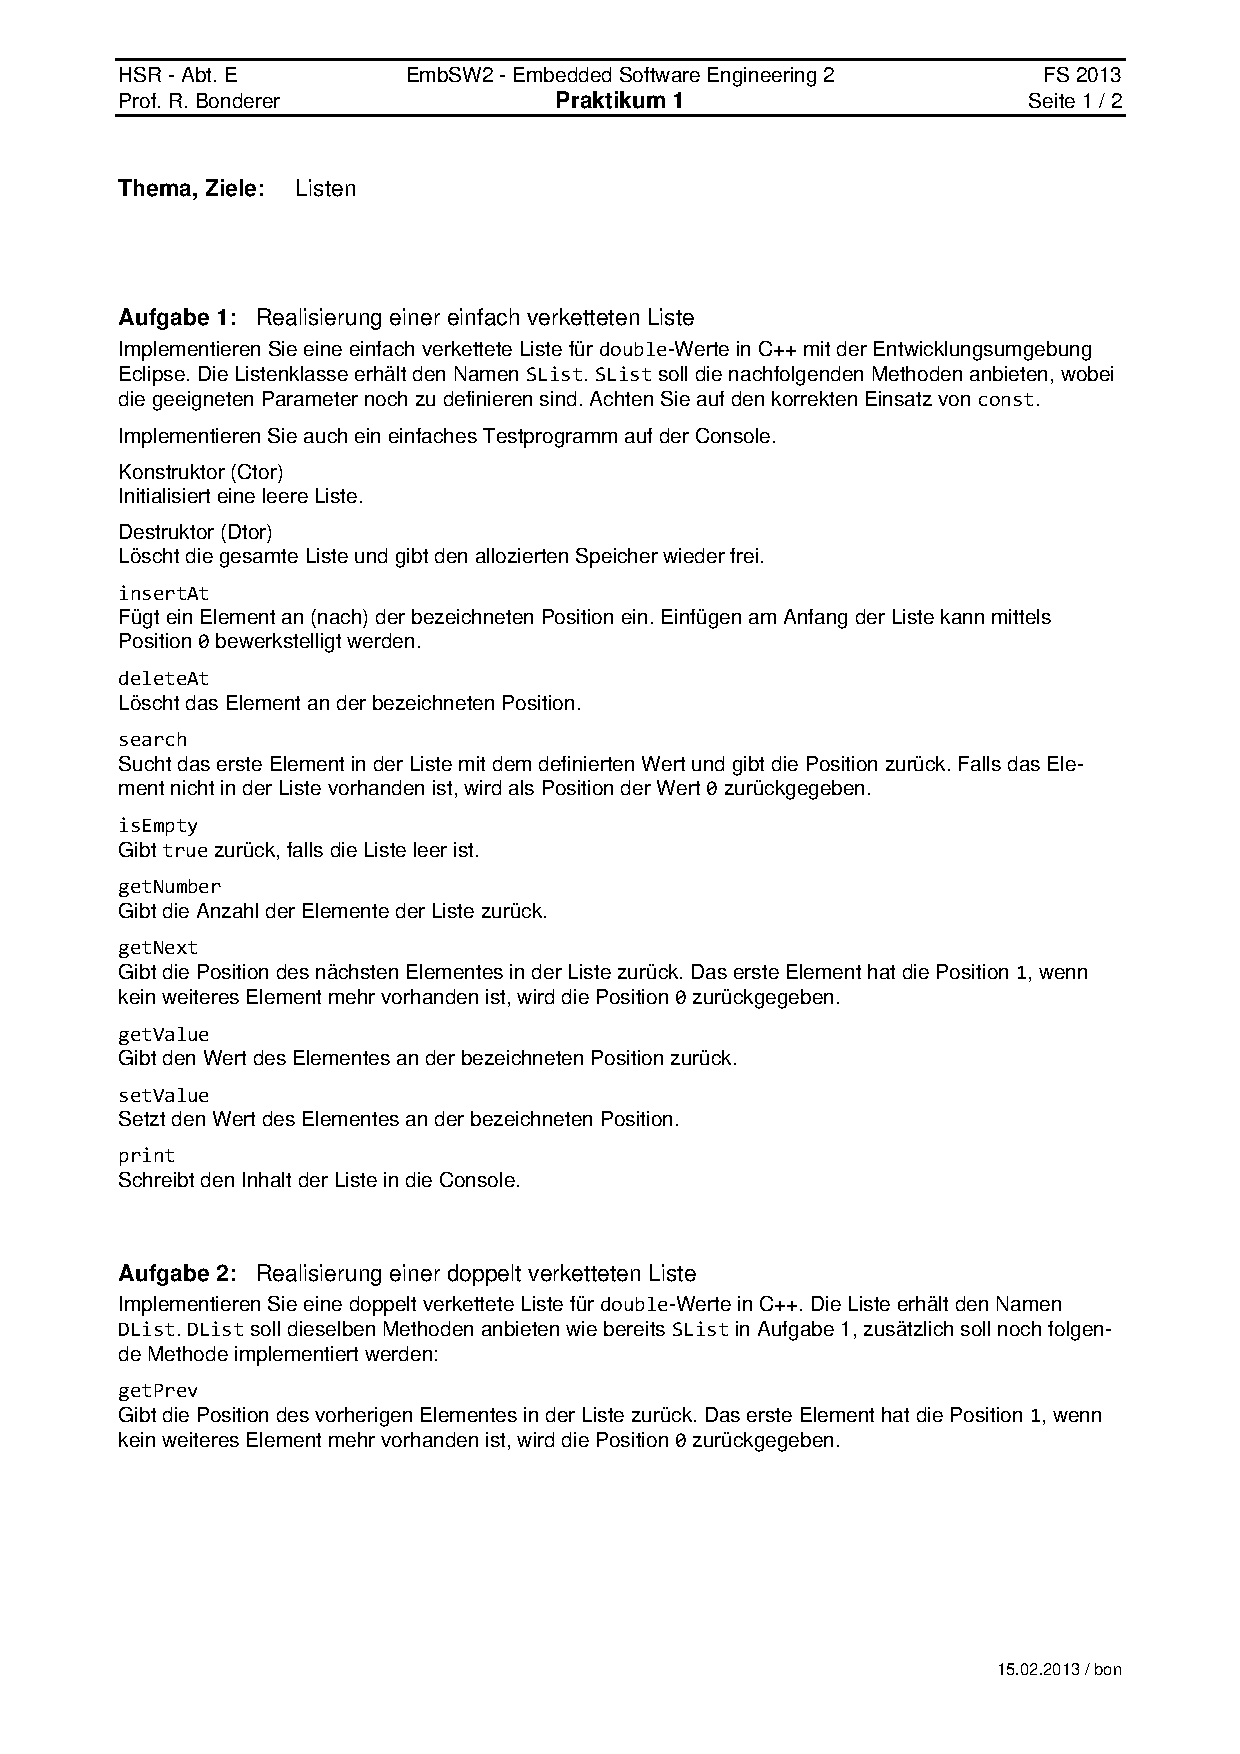
\includepdf[pages=-]{\basepath prak01/prak01.pdf}
\section{Praktikum 1 Lösungen}
\subsection{Aufgabe 1 \& 2}
\lstinputlisting{\basepath prak01/Loesung/Lists/src/Lists.cpp}
\lstinputlisting{\basepath prak01/Loesung/Lists/src/SList.h}
\lstinputlisting{\basepath prak01/Loesung/Lists/src/SList.cpp}
\lstinputlisting{\basepath prak01/Loesung/Lists/src/DList.h}
\lstinputlisting{\basepath prak01/Loesung/Lists/src/DList.cpp}
\subsection{Aufgabe 3}
\lstinputlisting{\basepath prak01/Loesung/A3/src/Lists.cpp}
\lstinputlisting{\basepath prak01/Loesung/A3/src/List.h}
\lstinputlisting{\basepath prak01/Loesung/A3/src/List.cpp}
\lstinputlisting{\basepath prak01/Loesung/A3/src/SList.h}
\lstinputlisting{\basepath prak01/Loesung/A3/src/SList.cpp}
\lstinputlisting{\basepath prak01/Loesung/A3/src/DList.h}
\lstinputlisting{\basepath prak01/Loesung/A3/src/DList.cpp}
\subsection{Aufgabe 4}
Man beachte, dass das protected Attribut \lstinline!nr! der Basisklasse mit dem Klassennamen qualifiziert werden
muss, d.h. \lstinline!List<T>::nr! statt einfach nur \lstinline!nr!. Ohne den Klassenqualifier kennt der Compiler das Attribut
nicht.
Die Methoden \lstinline!nodePtr()! wurden implizit inline in der Klassendeklaration definiert. Irgendwo klemmt der
Compiler, wenn die Definition im cpp-File gemacht wird. Der Code im cpp-File wurde mit \lstinline!#if 0 ... #endif!
auskommentiert.
\lstinputlisting{\basepath prak01/Loesung/A4/src/ListTest.cpp}
\lstinputlisting{\basepath prak01/Loesung/A4/src/List.h}
\lstinputlisting{\basepath prak01/Loesung/A4/src/List.cpp}
\lstinputlisting{\basepath prak01/Loesung/A4/src/SList.h}
\lstinputlisting{\basepath prak01/Loesung/A4/src/SList.cpp}
\lstinputlisting{\basepath prak01/Loesung/A4/src/DList.h}
\lstinputlisting{\basepath prak01/Loesung/A4/src/DList.cpp}

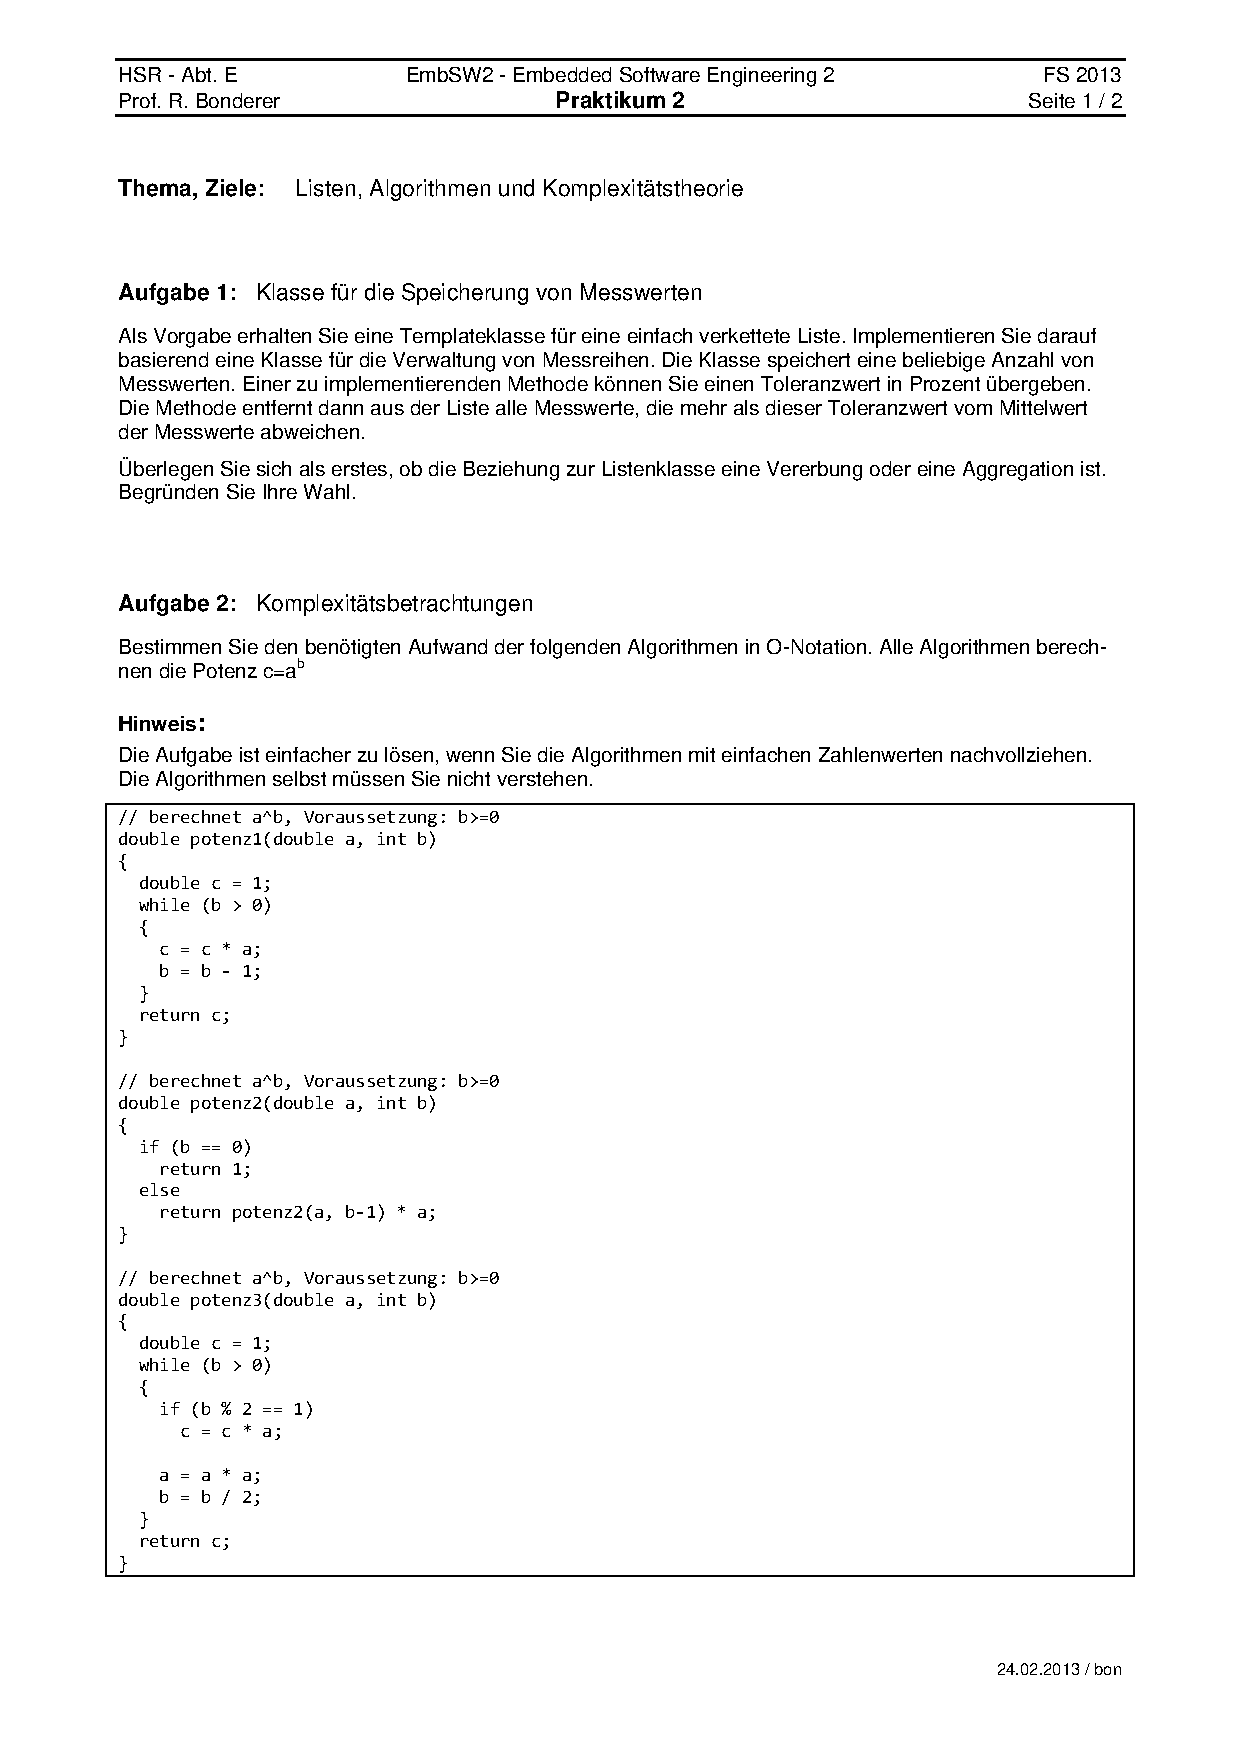
\includepdf[pages=-]{\basepath prak02/prak02.pdf}
\section{Praktikum 2 Lösungen}
\subsection{Aufgabe 1}
Die Messwertliste ist eine Liste, deshalb ist aus objektorientierter Sicht eine Vererbungsbeziehung vorzuziehen.
\lstinputlisting{\basepath prak02/Loesung/MeasureListInh/src/MListMain.cpp}
\lstinputlisting{\basepath prak02/Loesung/MeasureListInh/src/MeasureList.h}
\lstinputlisting{\basepath prak02/Loesung/MeasureListInh/src/MeasureList.cpp}
Die Lösung mit einer Aggregation ist ebenfalls möglich:
\lstinputlisting{\basepath prak02/Loesung/MeasureListAgg/src/MListMain.cpp}
\lstinputlisting{\basepath prak02/Loesung/MeasureListAgg/src/MeasureList.h}
\lstinputlisting{\basepath prak02/Loesung/MeasureListAgg/src/MeasureList.cpp}
\subsection{Aufgabe 2}
In der Funktion \lstinline!potenz1()! wird die while-Schleife b mal durchlaufen, d.h. dieser Algorithmus ist $O(b)$.
Die Funktion \lstinline!potenz2()! wird b mal rekursiv aufgerufen, weitere Schleifen sind nicht vorhanden, d.h. dieser
Algorithmus ist $O(b)$.
In der Funktion \lstinline!potenz3()! wird b bei jedem Schleifendurchlauf halbiert. Die Schleife wird ungefähr ld(b)
mal durchlaufen (ld = logarithmus dualis, Zweierlogarithmus). \lstinline!potenz3()! ist demnach $O(log b)$.
\subsection{Aufgabe 3}
Der Stack ist keine Liste, er benutzt nur eine für die Speicherung der Daten. Eine Vererbung kommt deshalb
nicht in Frage, Aggregation ist die richtige Variante. Da der Stack beliebige Daten speichern können soll,
muss er unbedingt als Templateklasse implementiert werden.
\lstinputlisting{\basepath prak02/Loesung/DynaStack/stacktest.cpp}
\lstinputlisting{\basepath prak02/Loesung/DynaStack/StackUI.h}
\lstinputlisting{\basepath prak02/Loesung/DynaStack/StackUI.cpp}
\lstinputlisting{\basepath prak02/Loesung/DynaStack/stack.h}
\lstinputlisting{\basepath prak02/Loesung/DynaStack/stack.cpp}

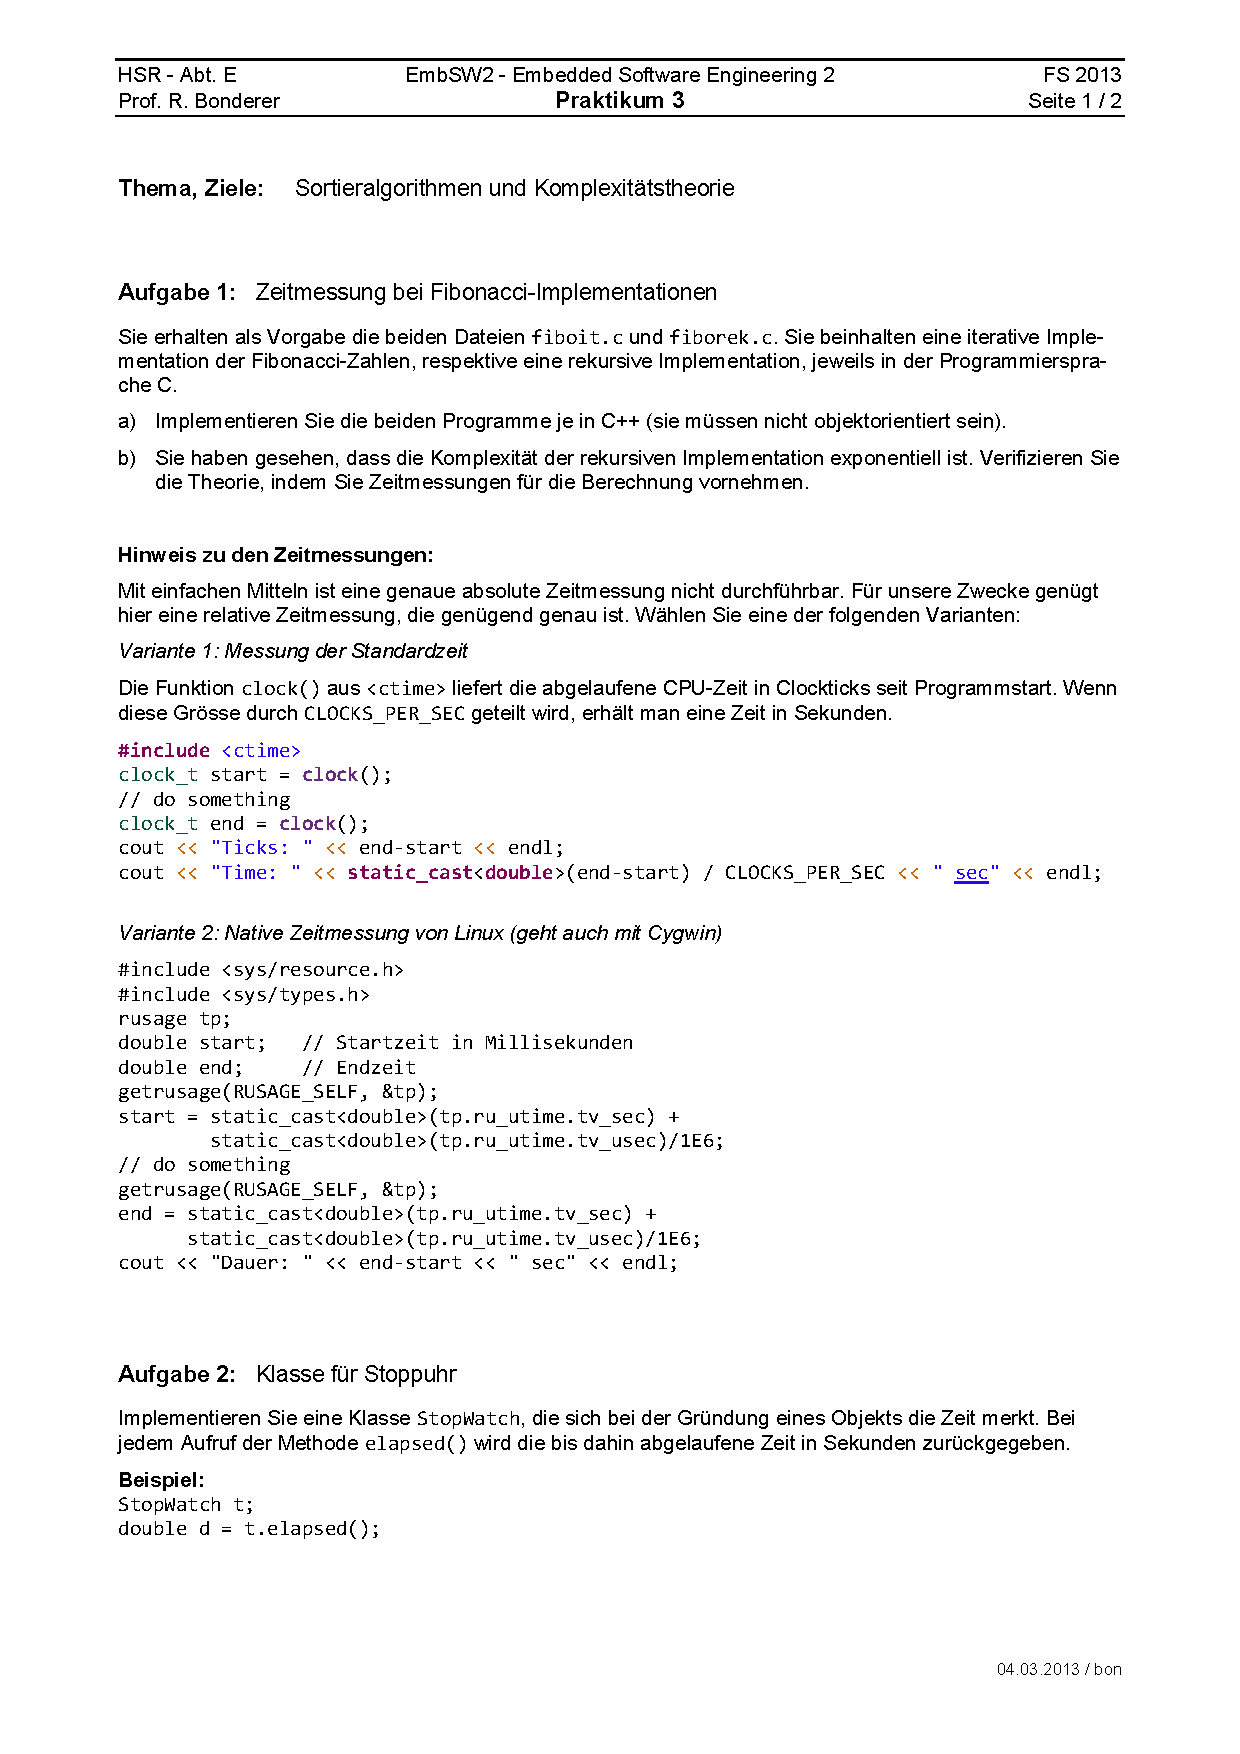
\includepdf[pages=-]{\basepath prak03/prak03.pdf}
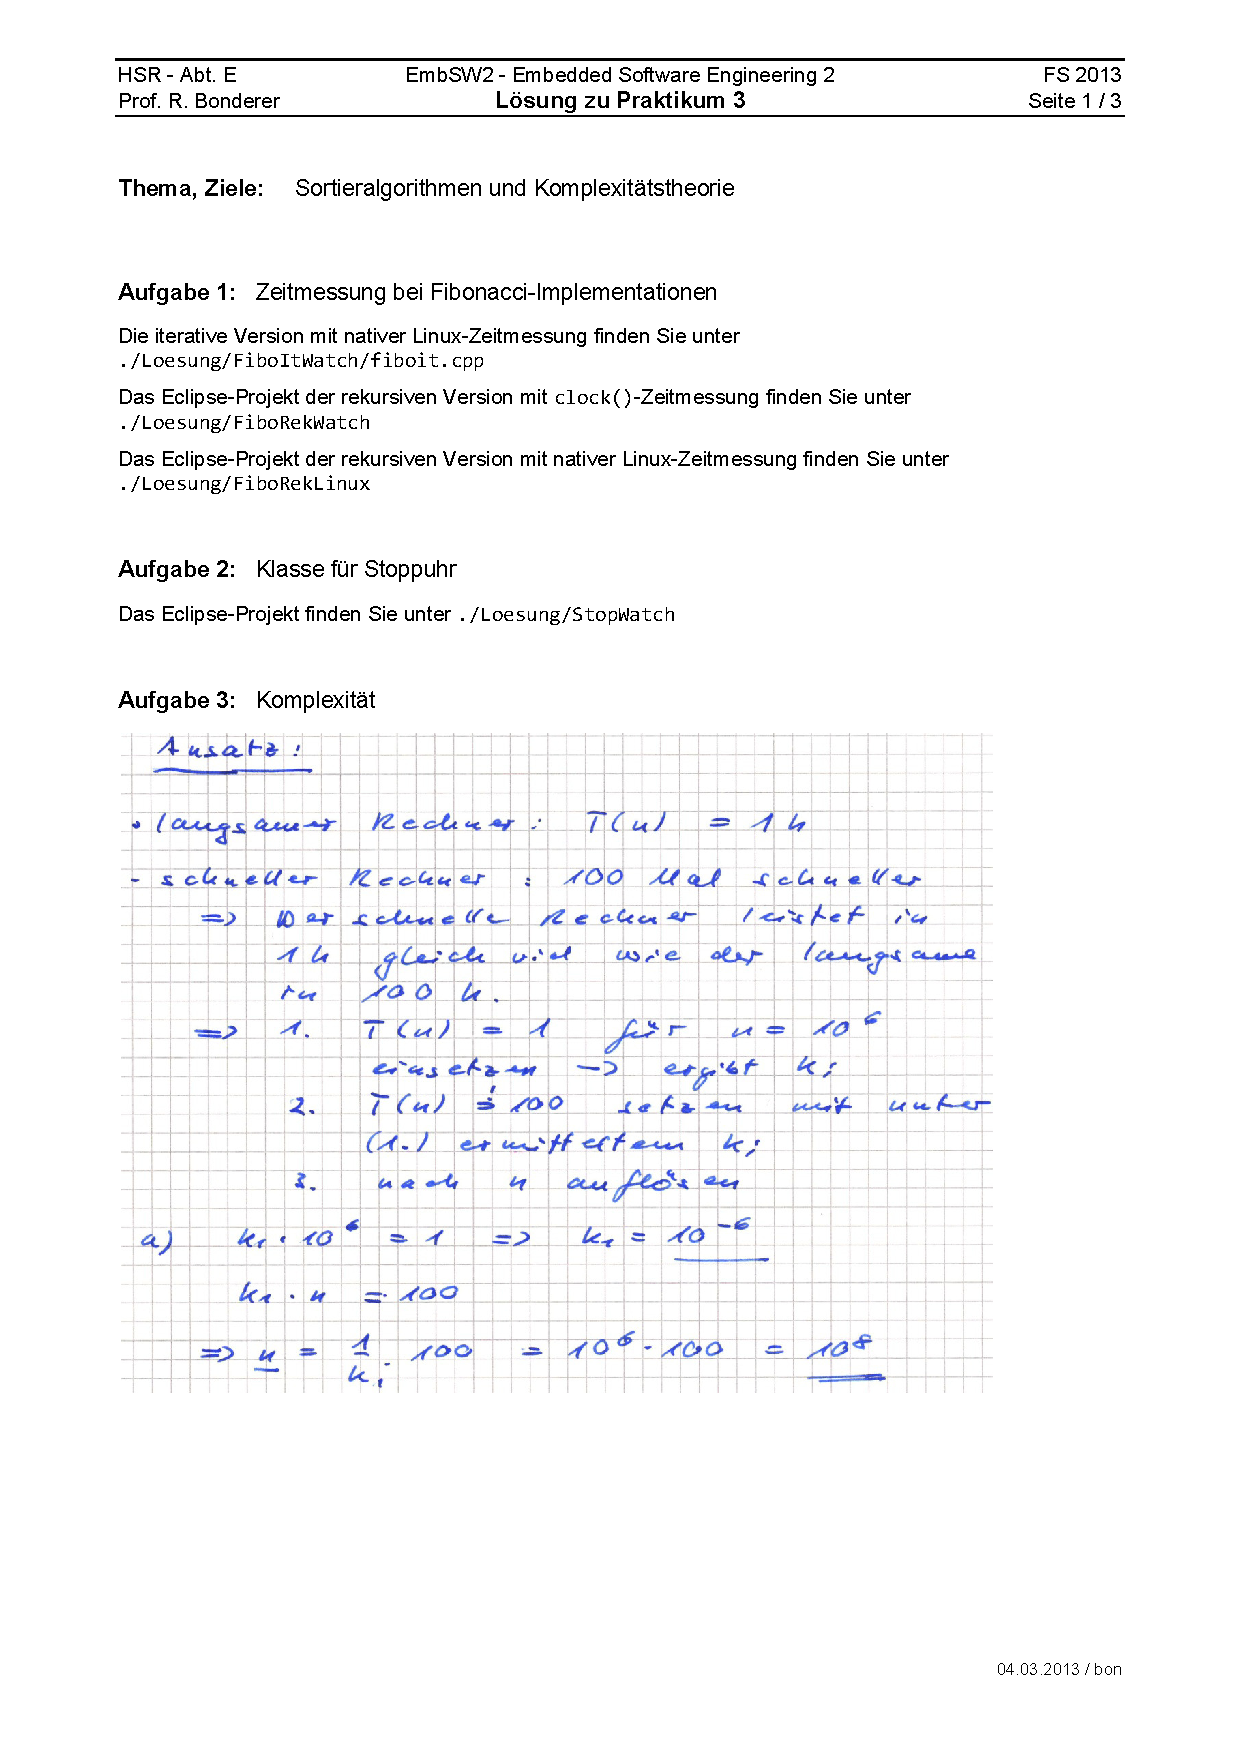
\includepdf[pages=-]{\basepath prak03/loesung03.pdf}
\section{Praktikum 3 Lösungen}
\subsection{Aufgabe 1}
\lstinputlisting{\basepath prak03/Loesung/FiboItWatch/fiboit.cpp}
\lstinputlisting{\basepath prak03/Loesung/FiboRekWatch/fiborek.cpp}
\subsection{Aufgabe 2}
\lstinputlisting{\basepath prak03/Loesung/StopWatch/src/StopWatchTest.cpp}
\lstinputlisting{\basepath prak03/Loesung/StopWatch/src/StopWatch.h}
\lstinputlisting{\basepath prak03/Loesung/StopWatch/src/StopWatch.cpp}
\subsection{Aufgabe 3}
Siehe Lösungs-PDF!
\subsection{Aufgabe 4}
Siehe Lösungs-PDF!
\lstinputlisting{\basepath prak03/Loesung/QuickSortFast/src/QuickSortFast.cpp}


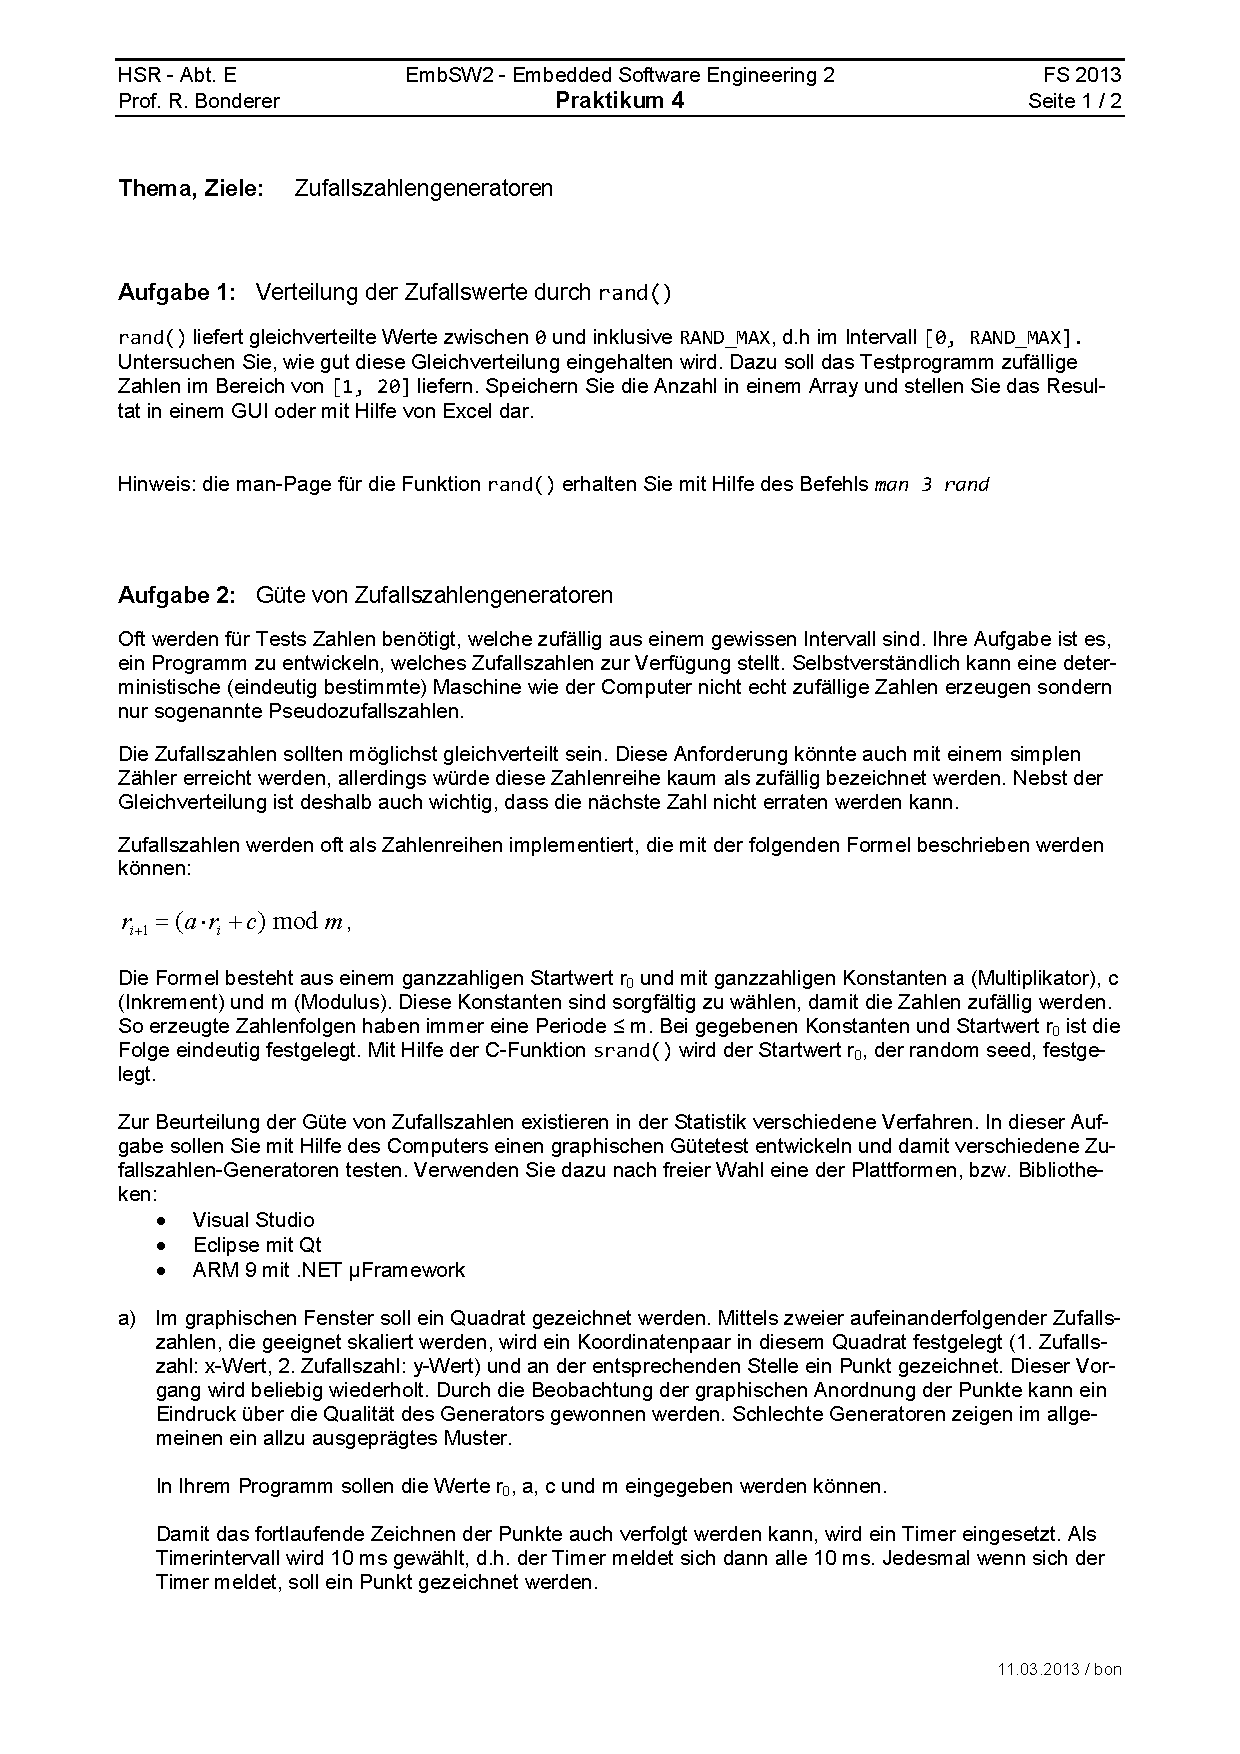
\includepdf[pages=-]{\basepath prak04/prak04.pdf}
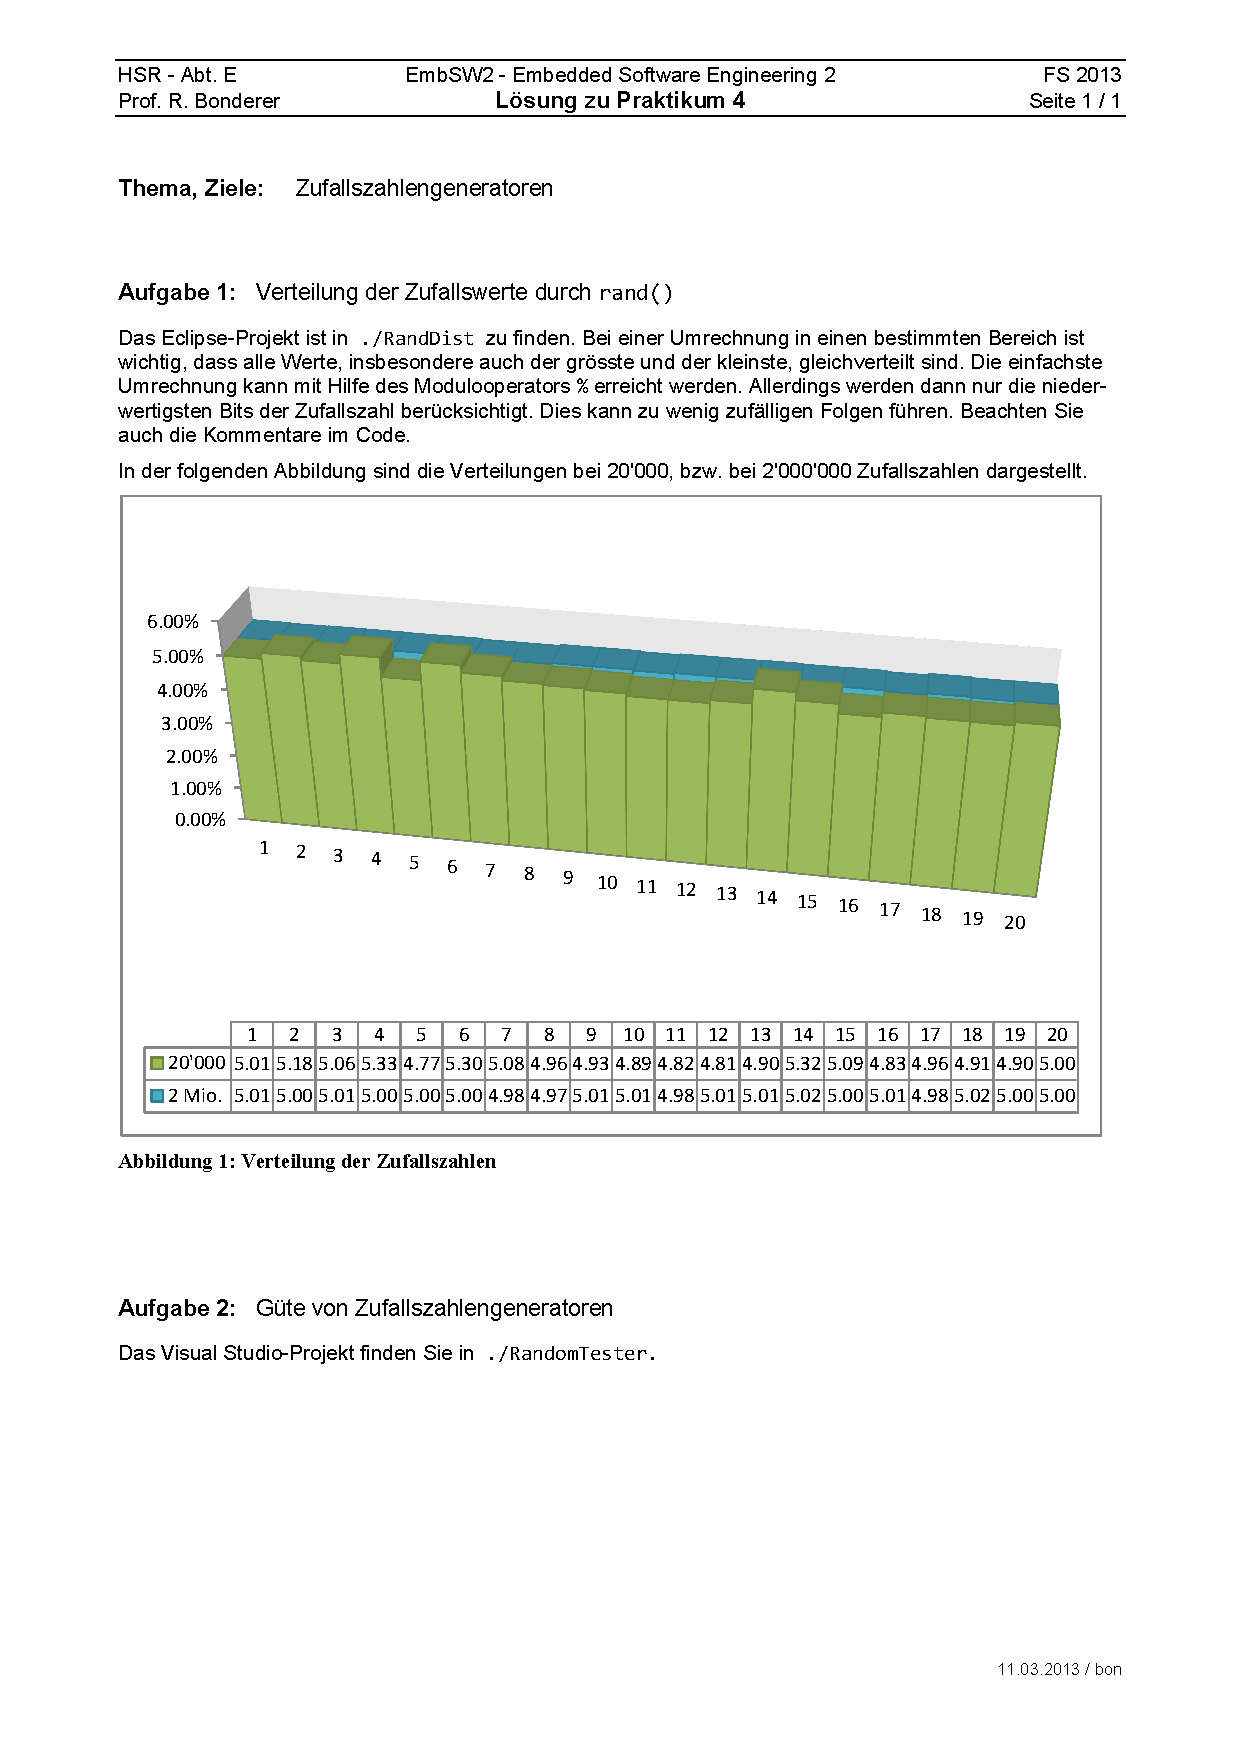
\includepdf[pages=-]{\basepath prak04/loesung04.pdf}
\section{Praktikum 4 Lösungen}
\subsection{Aufgabe 1}
Siehe Lösungs-PDF!
\subsection{Aufgabe 2}
\lstinputlisting{\basepath prak04/RandDist/src/RandDist.cpp}


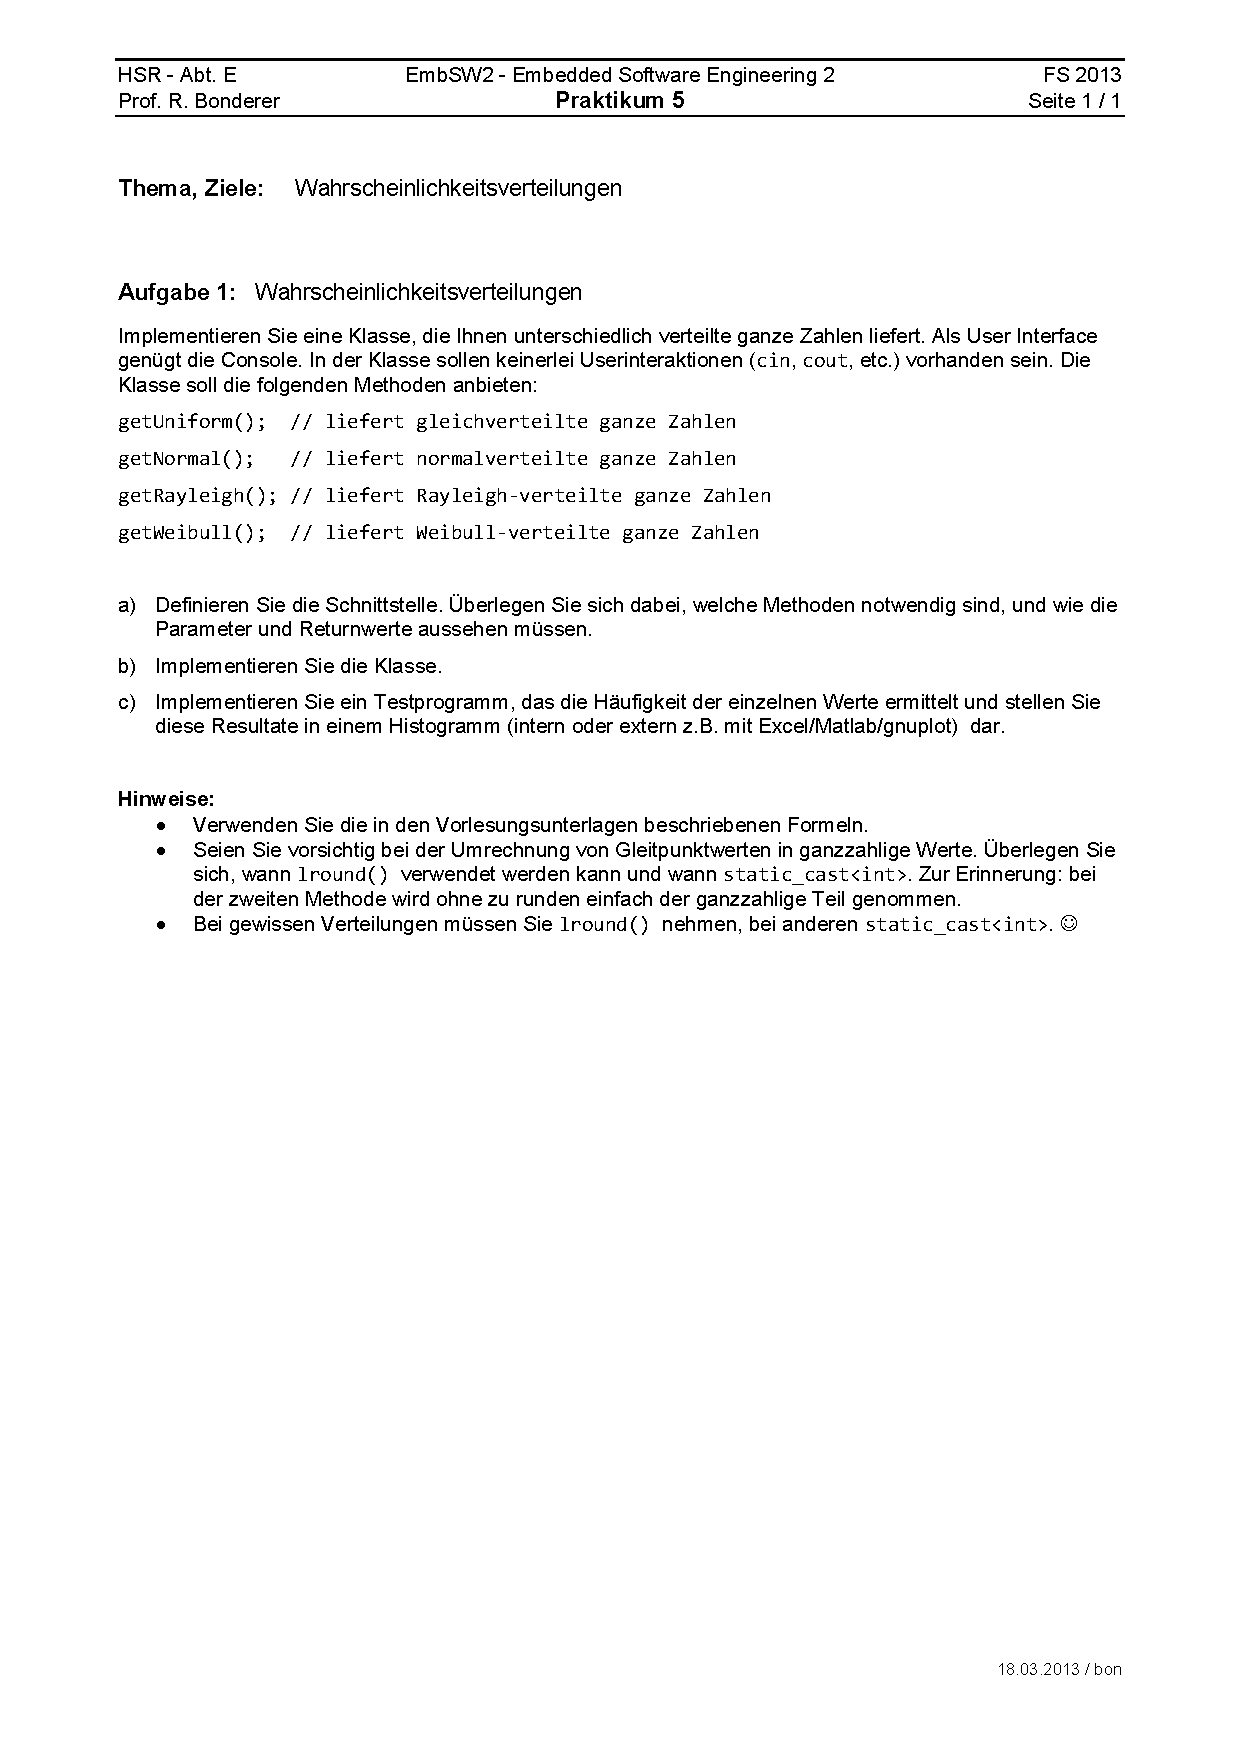
\includepdf[pages=-]{\basepath prak05/prak05.pdf}
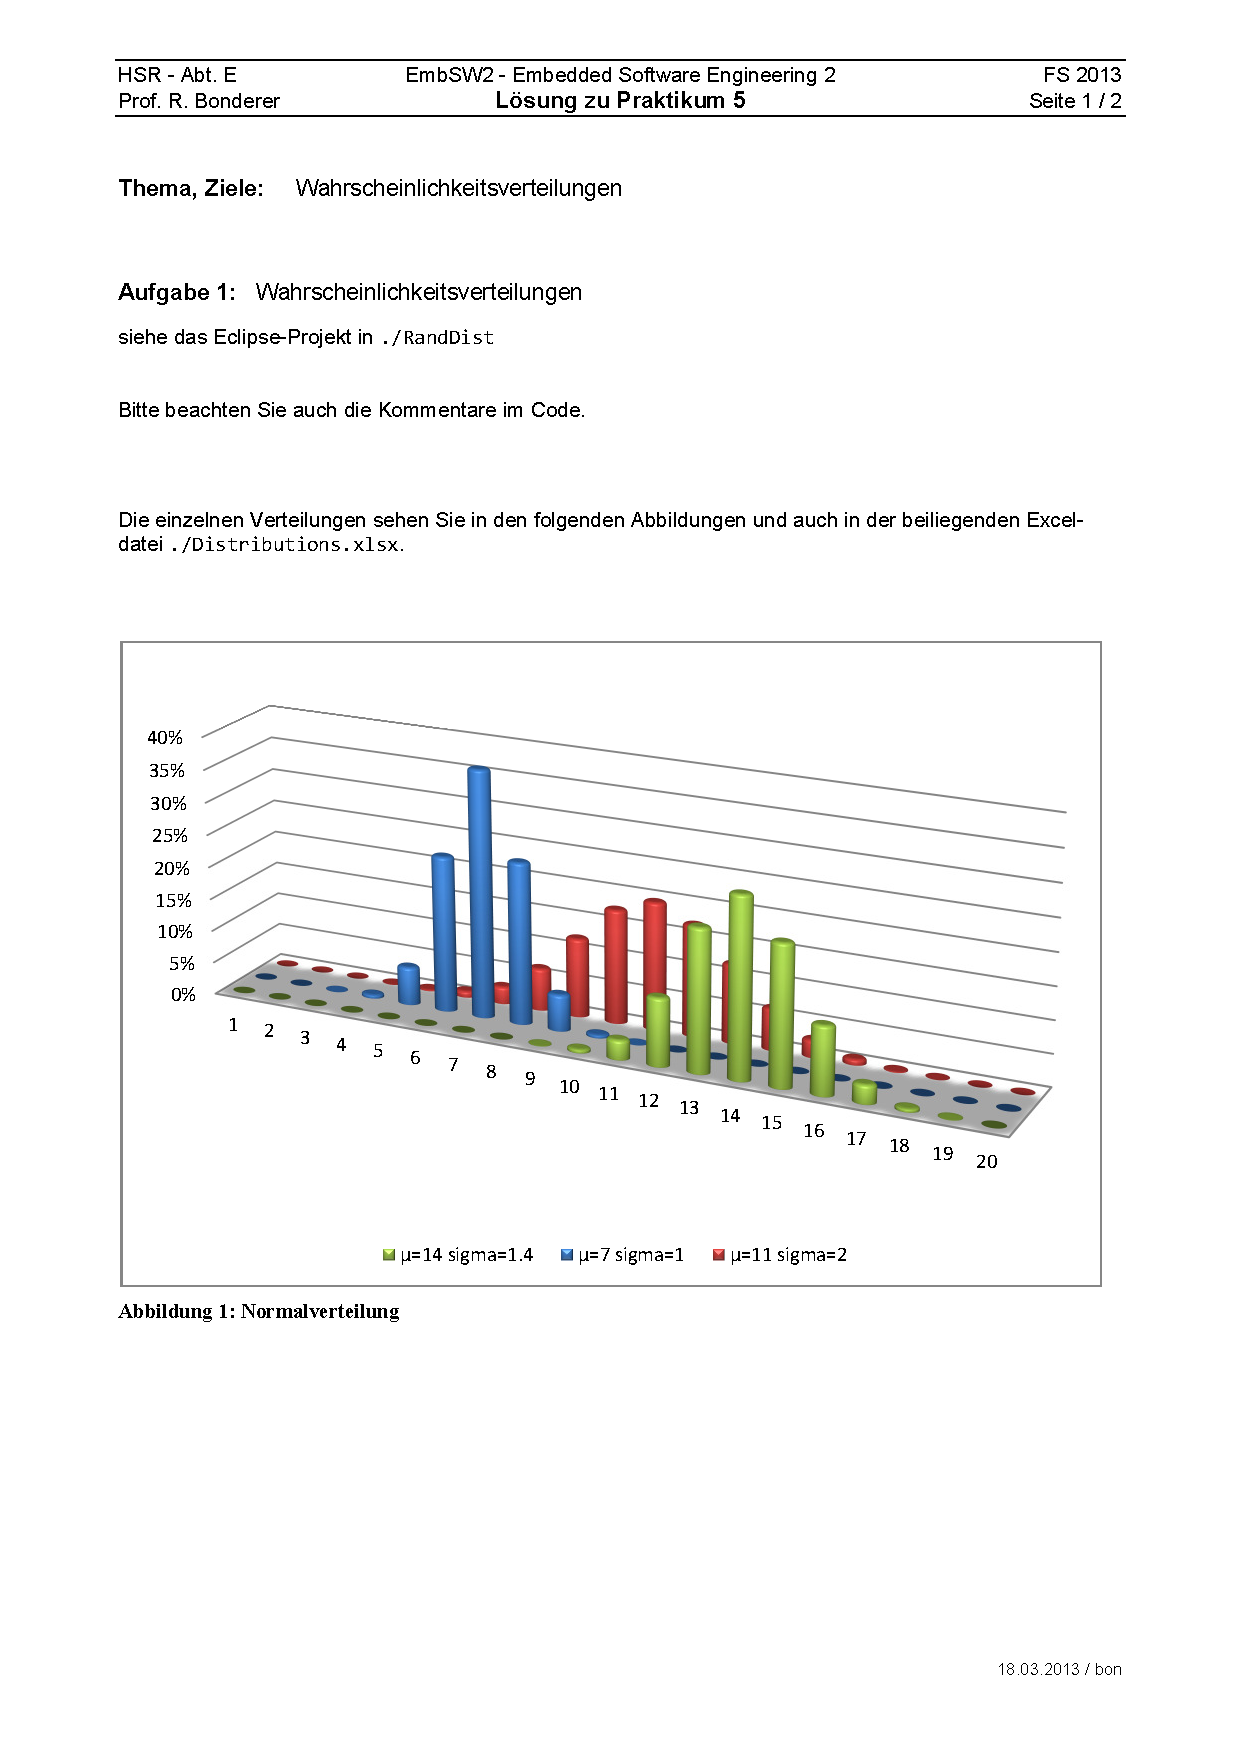
\includepdf[pages=-]{\basepath prak05/loesung05.pdf}
\section{Praktikum 5 Lösungen}
\subsection{Aufgabe 1}
\lstinputlisting{\basepath prak05/RandDist/src/RandDist.cpp}
\lstinputlisting{\basepath prak05/RandDist/src/Randgen.h}
\lstinputlisting{\basepath prak05/RandDist/src/Randgen.cpp}


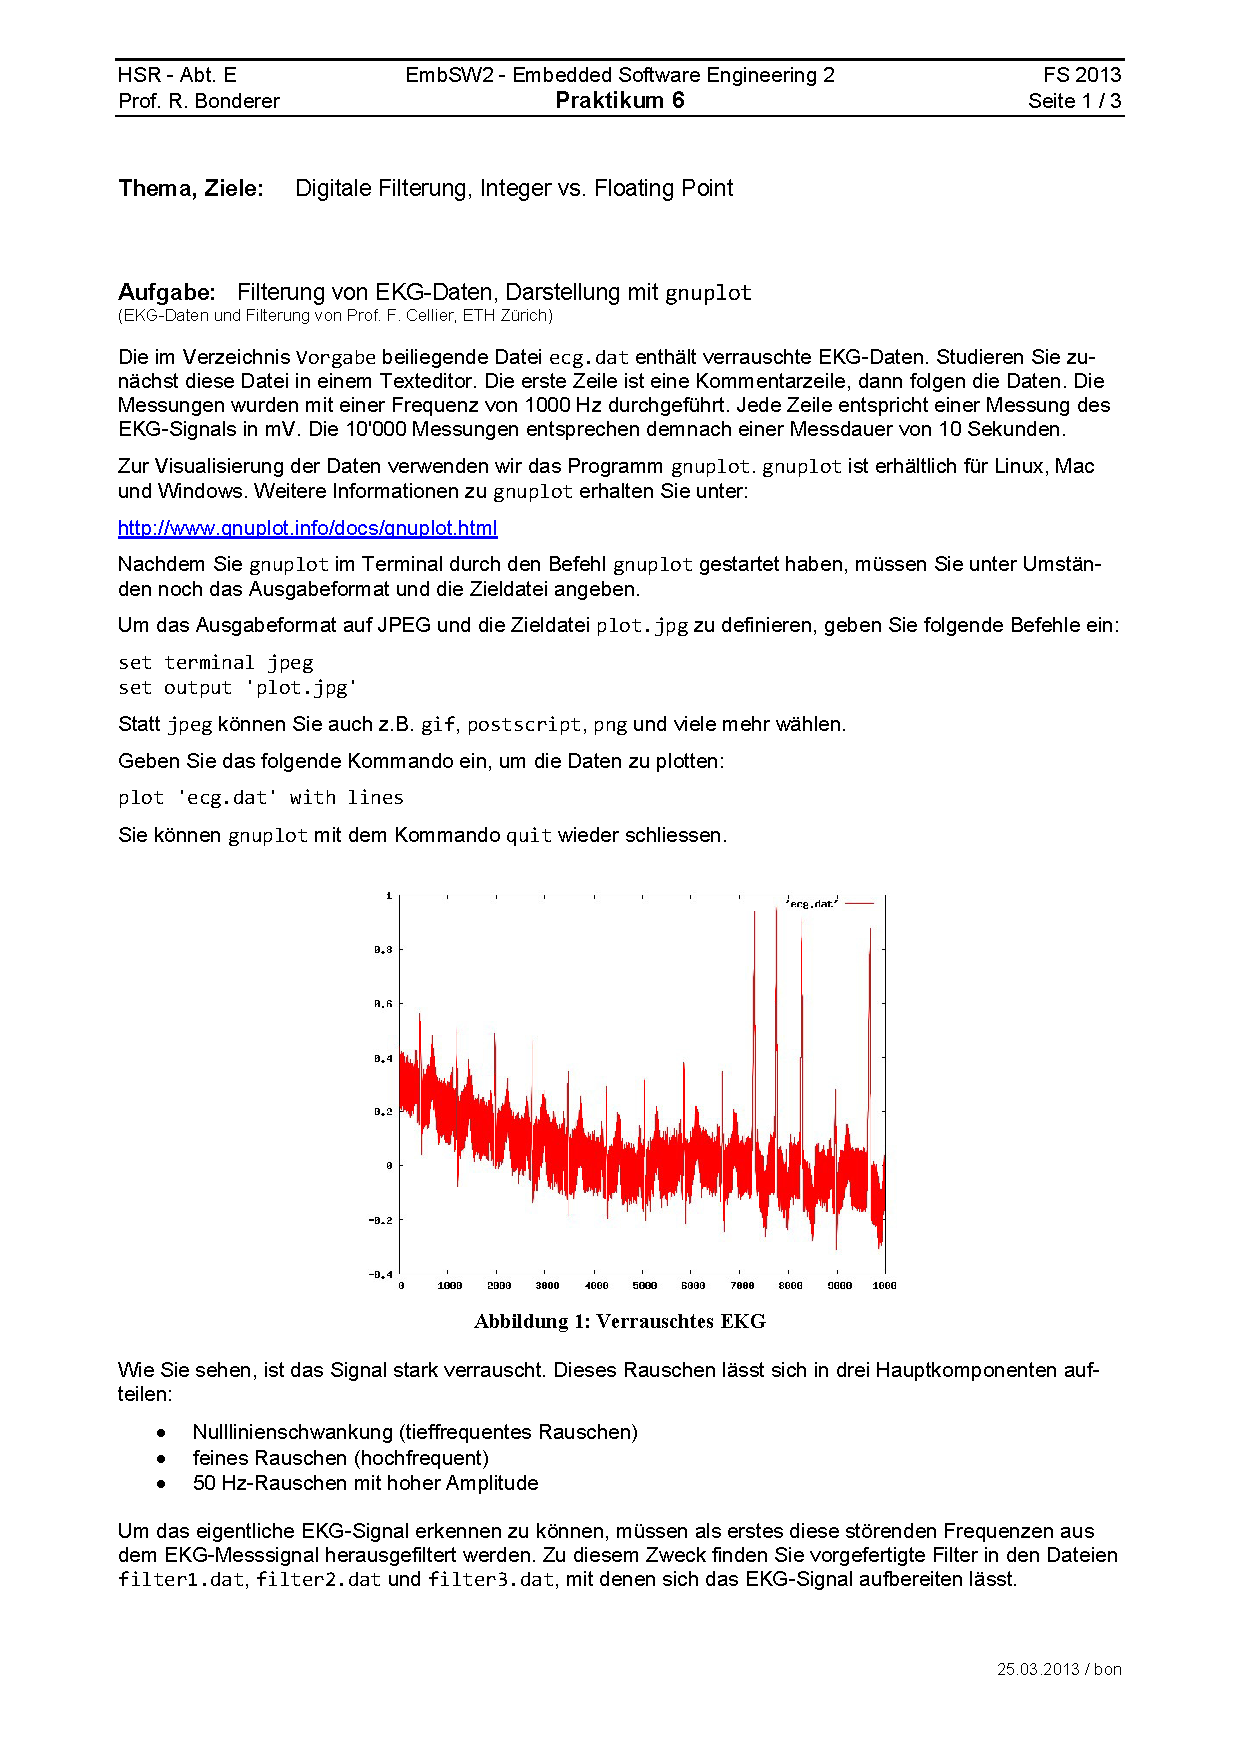
\includepdf[pages=-]{\basepath prak06/prak06.pdf}
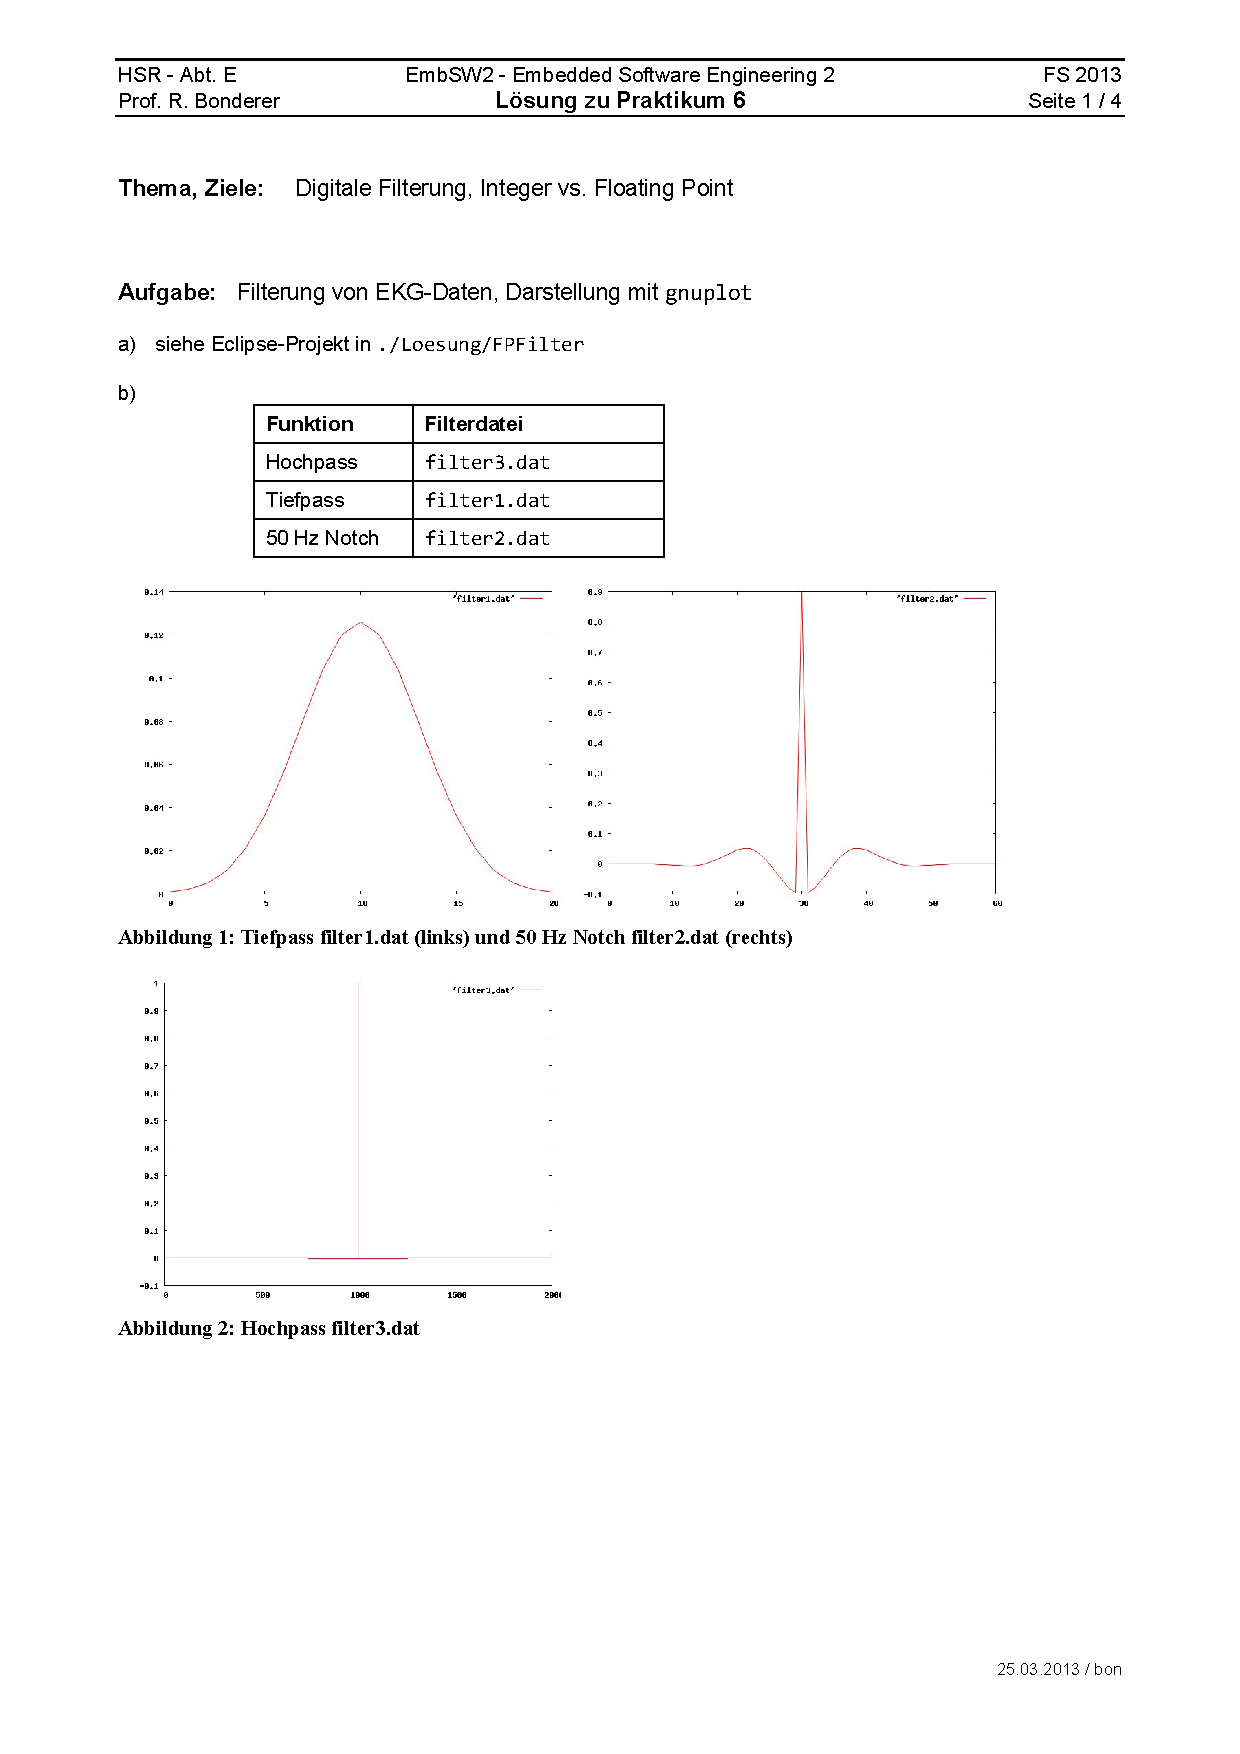
\includepdf[pages=-]{\basepath prak06/loesung06.pdf}
\section{Praktikum 6 Lösungen}
\lstinputlisting{\basepath prak06/Loesung/FPFilter/fpfiltertest.cpp}
\lstinputlisting{\basepath prak06/Loesung/FPFilter/fpfilter.h}
\lstinputlisting{\basepath prak06/Loesung/FPFilter/fpfilter.cpp}

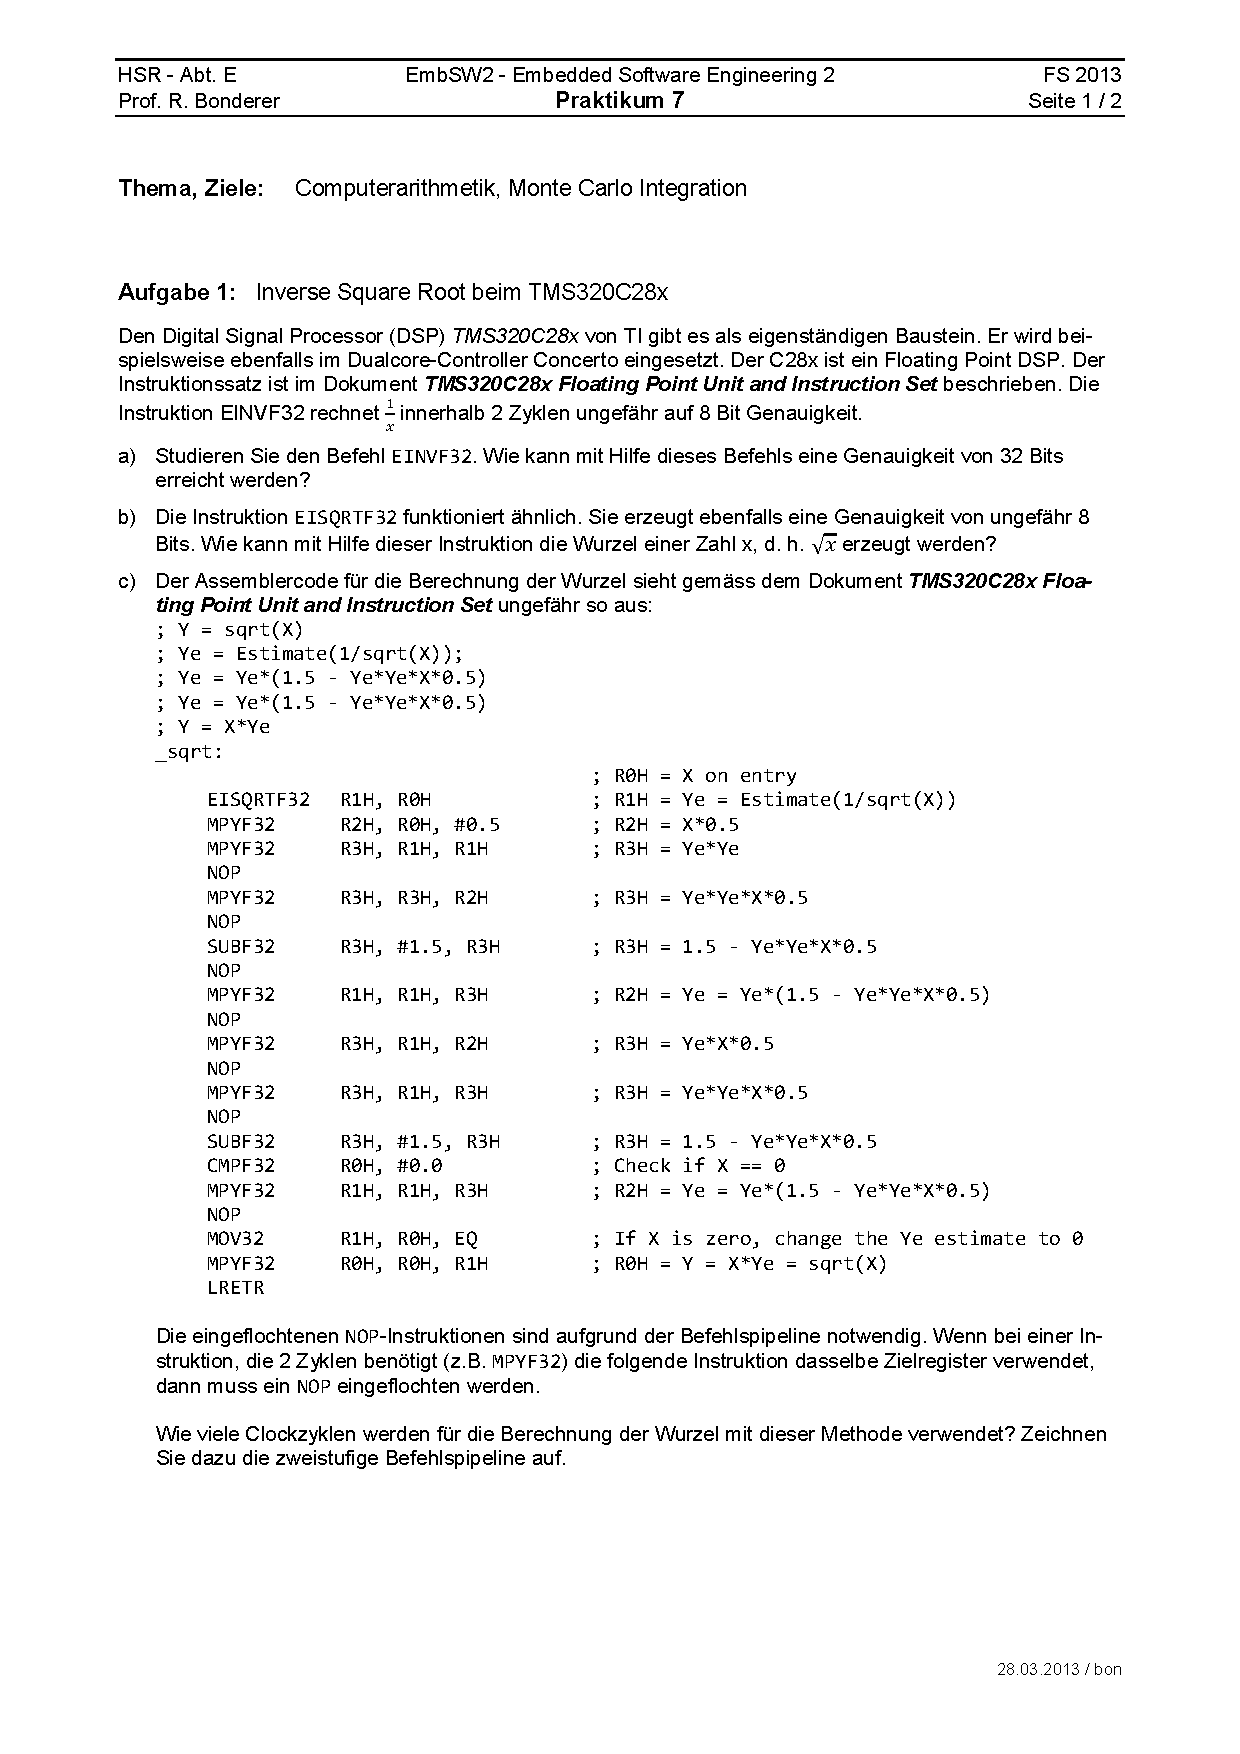
\includepdf[pages=-]{\basepath prak07/prak07.pdf}
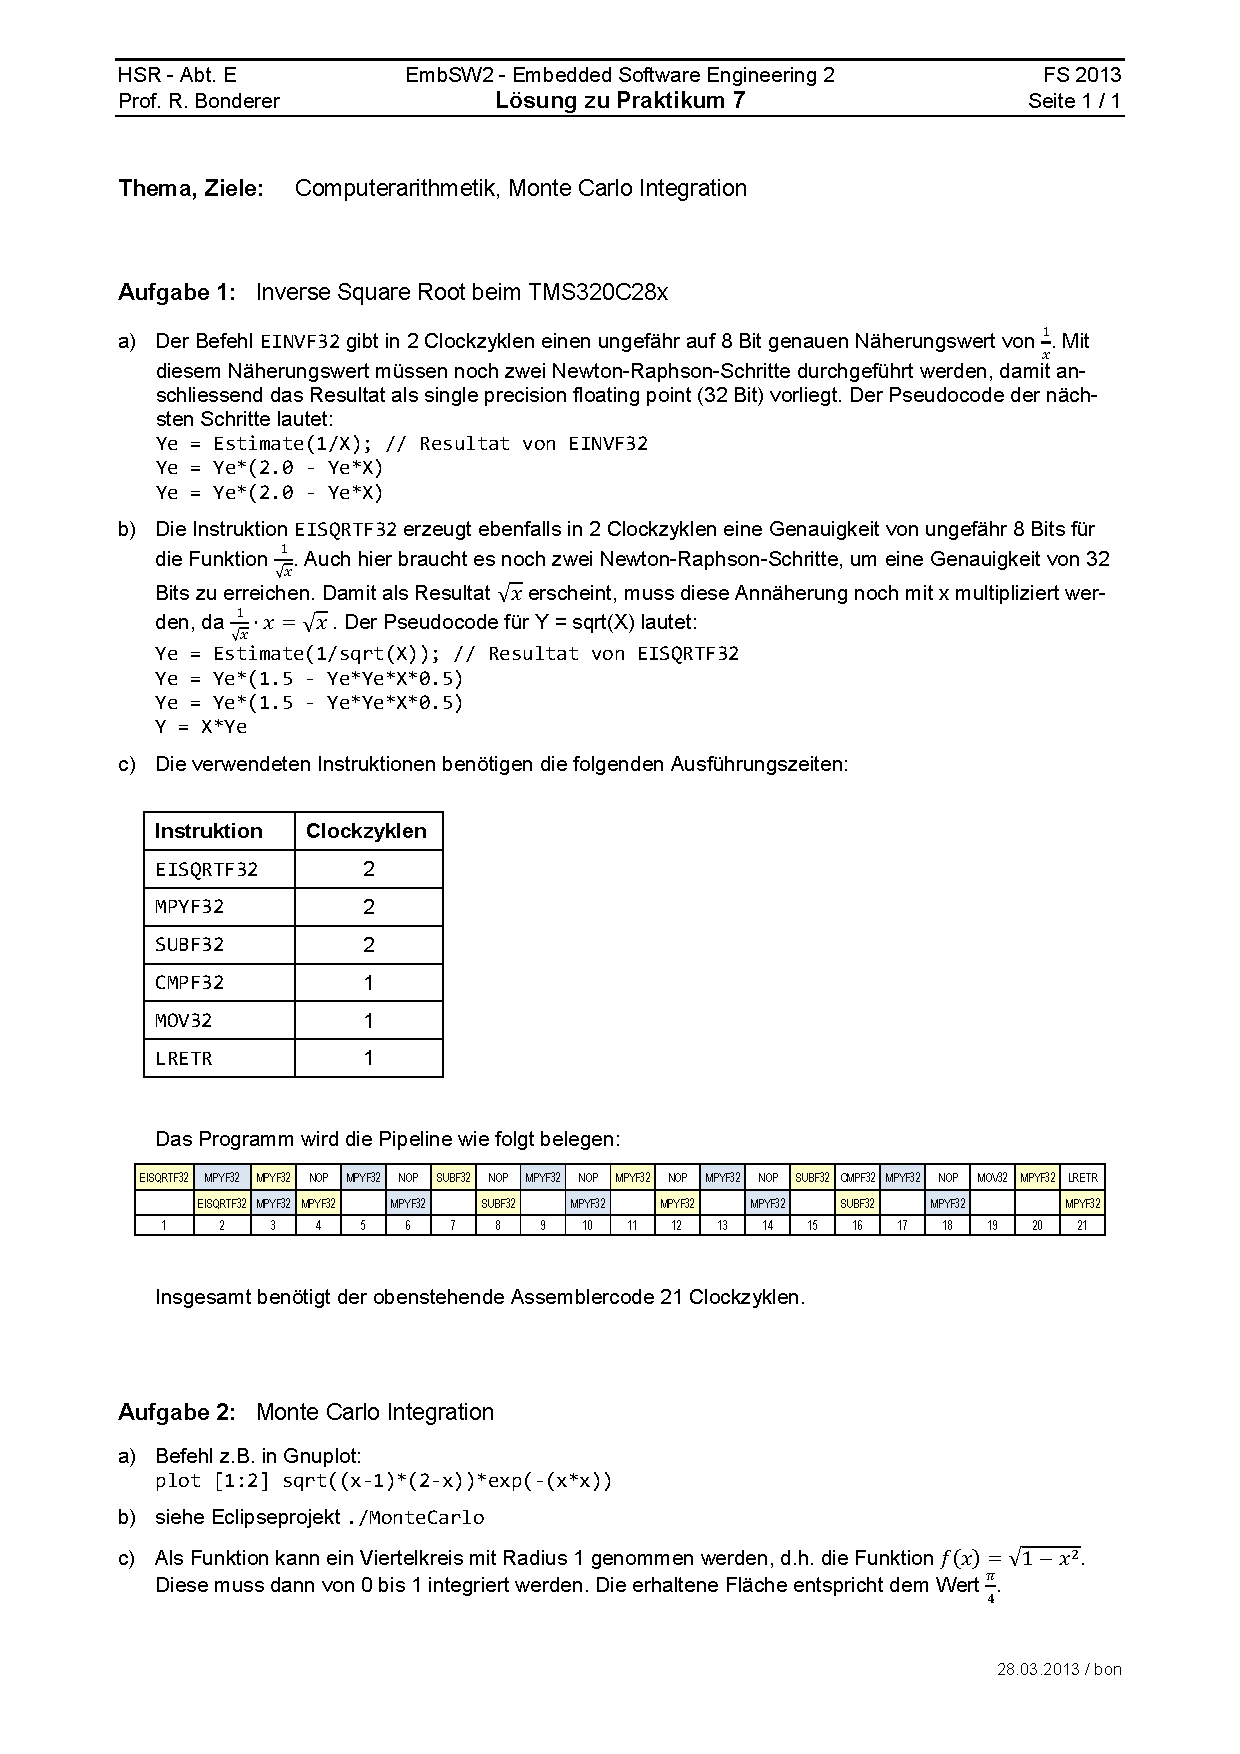
\includepdf[pages=-]{\basepath prak07/loesung07.pdf}
\section{Praktikum 7 Lösungen}
\lstinputlisting{\basepath prak07/MonteCarlo/main.cpp}
\lstinputlisting{\basepath prak07/MonteCarlo/montecarlo.h}
\lstinputlisting{\basepath prak07/MonteCarlo/montecarlo.cpp}


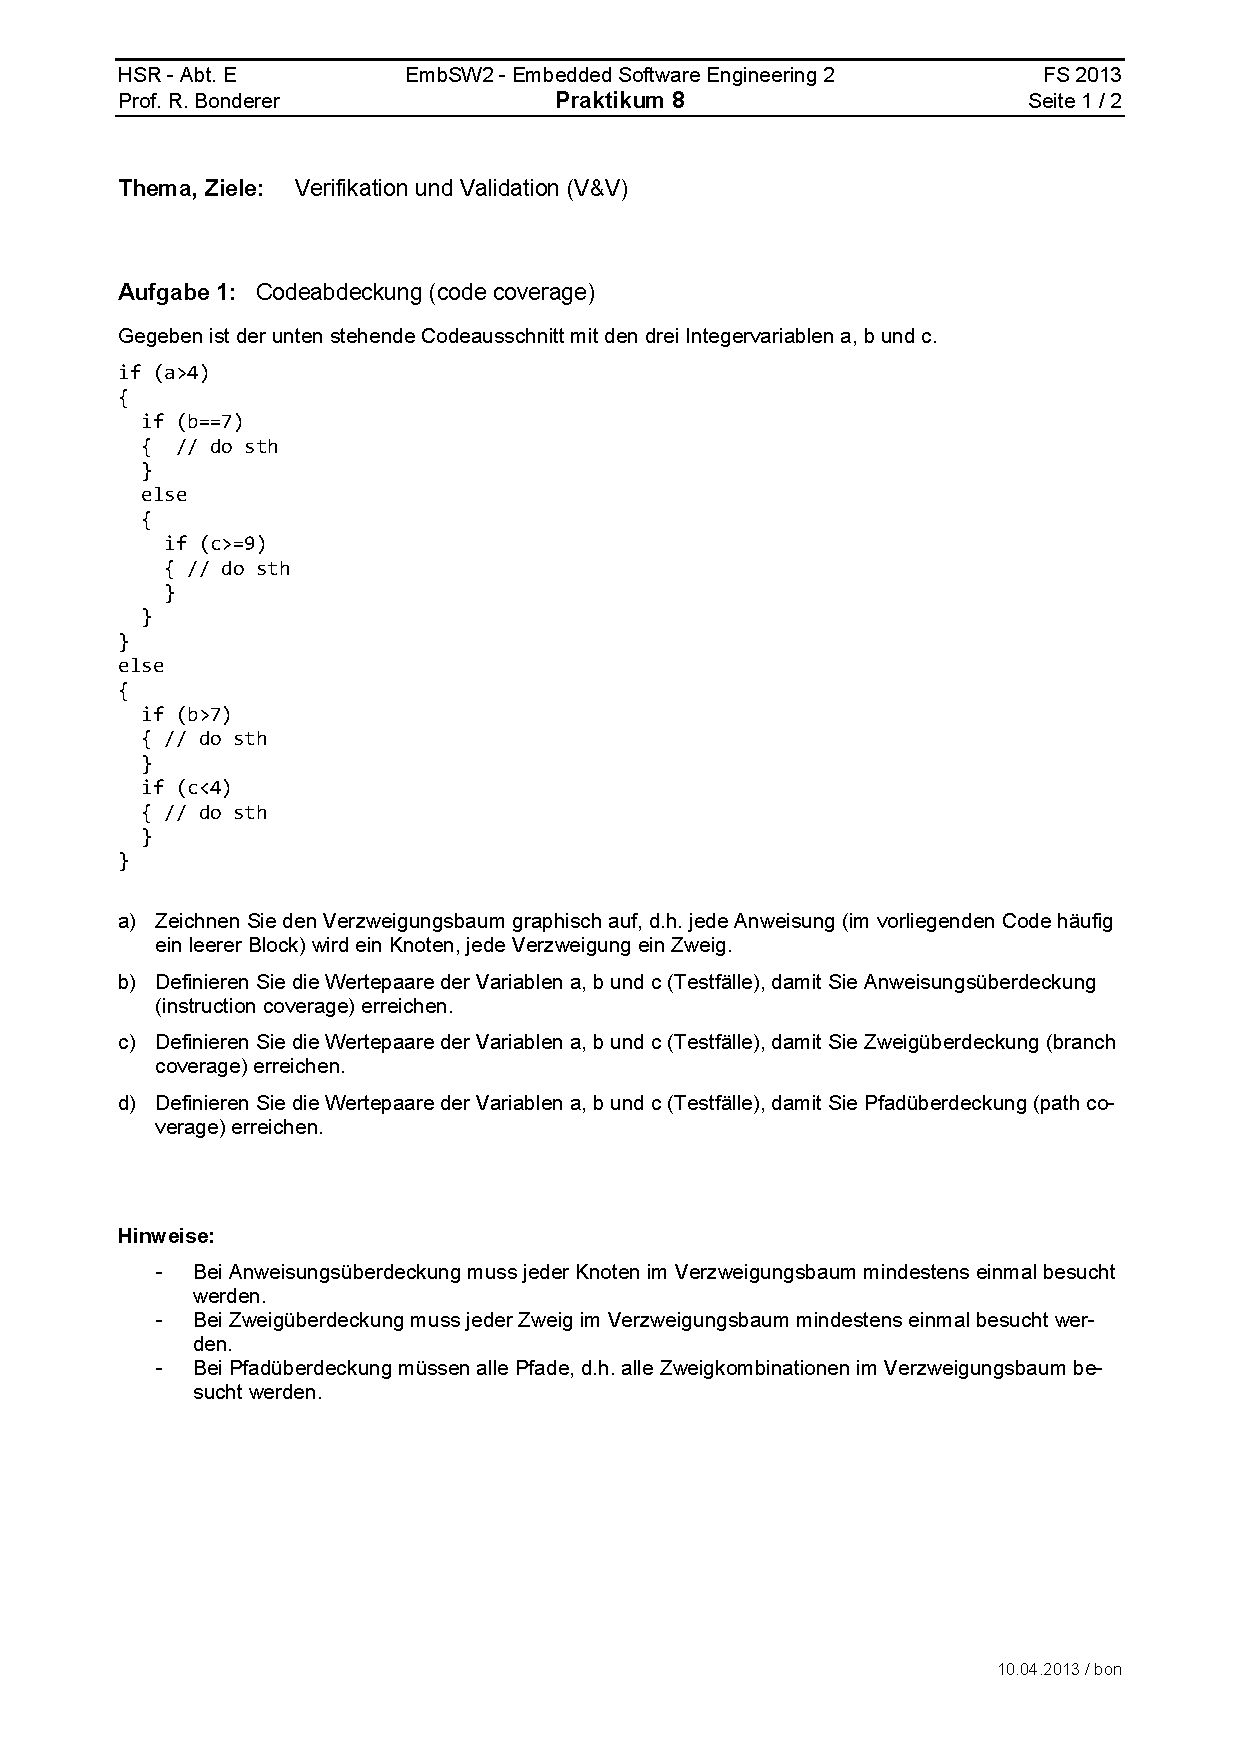
\includepdf[pages=-]{\basepath prak08/prak08.pdf}
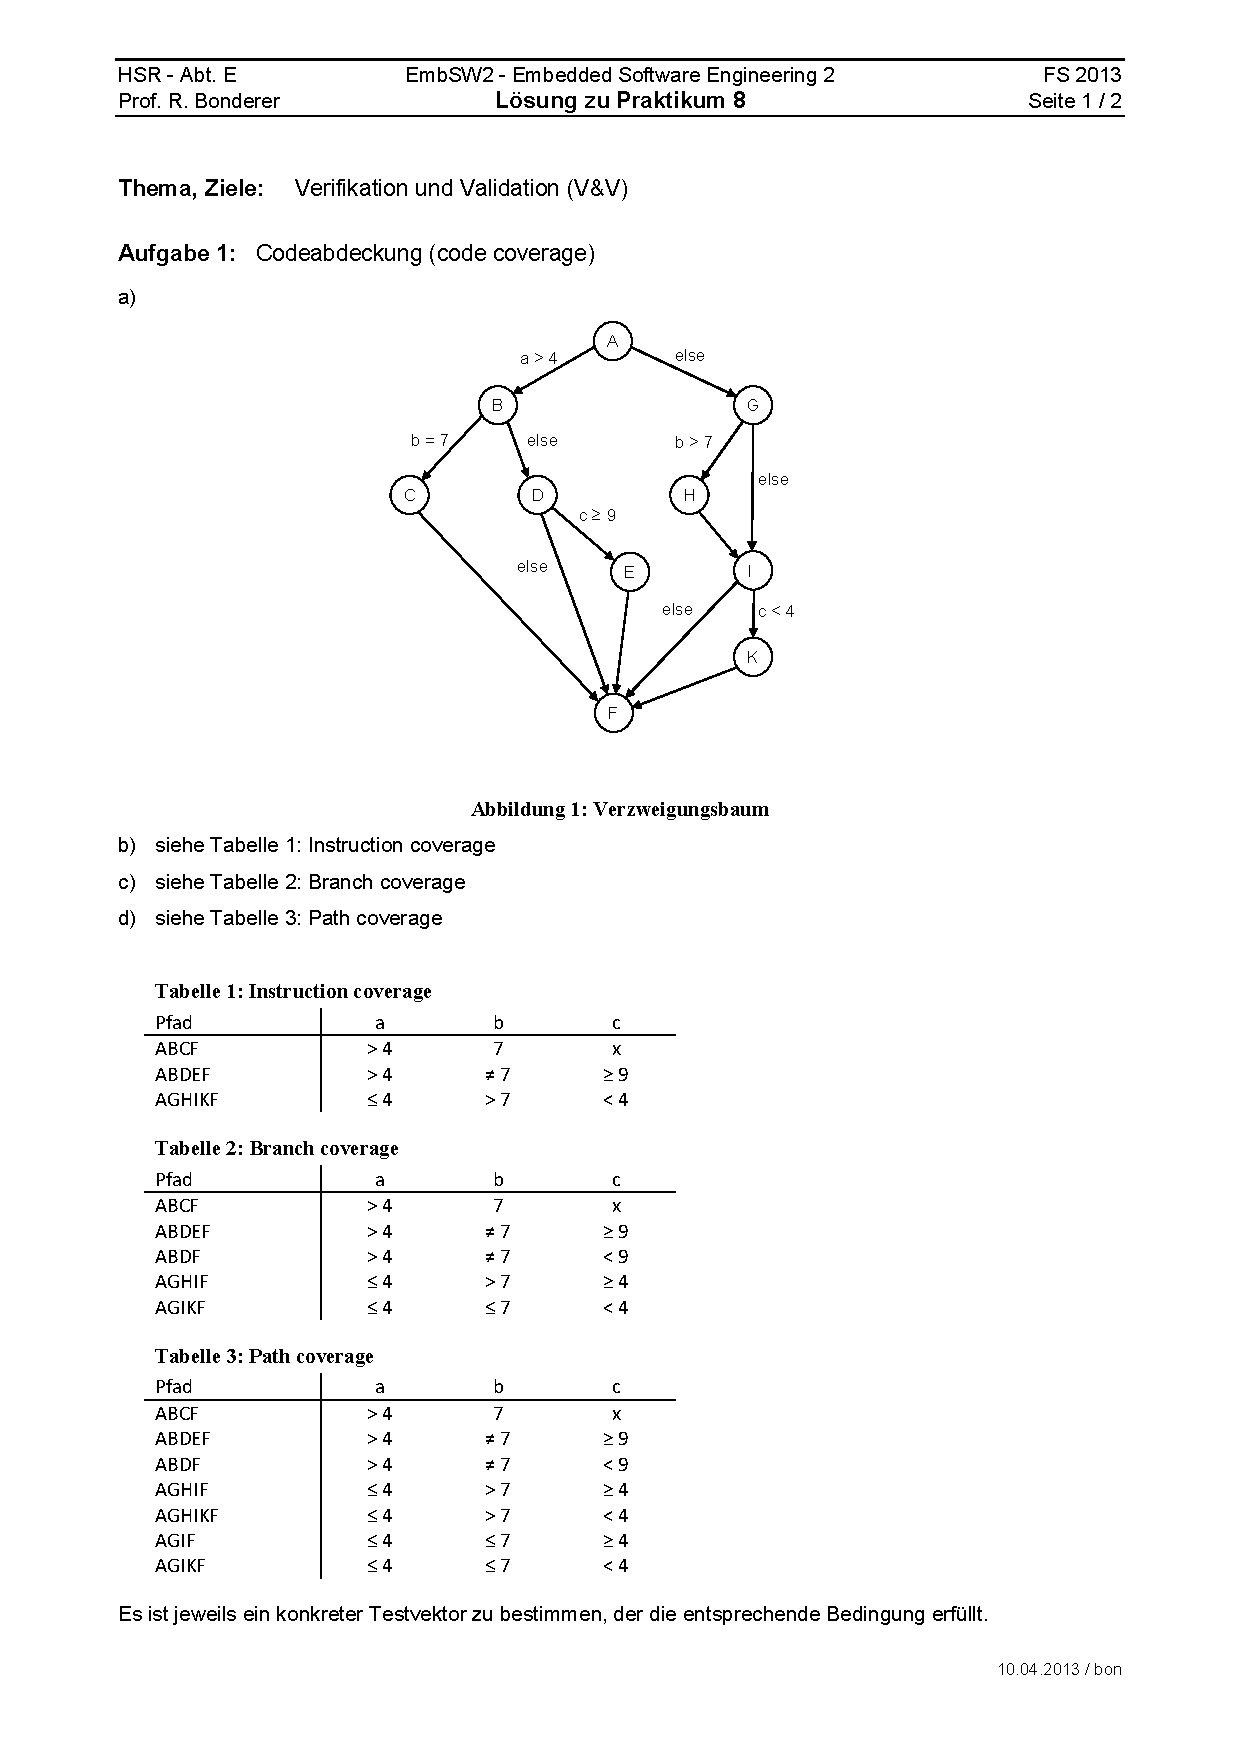
\includepdf[pages=-]{\basepath prak08/loesung08.pdf}
\section{Praktikum 8 Lösungen}
\lstinputlisting{\basepath prak08/Loesung/Correct/main.cpp}

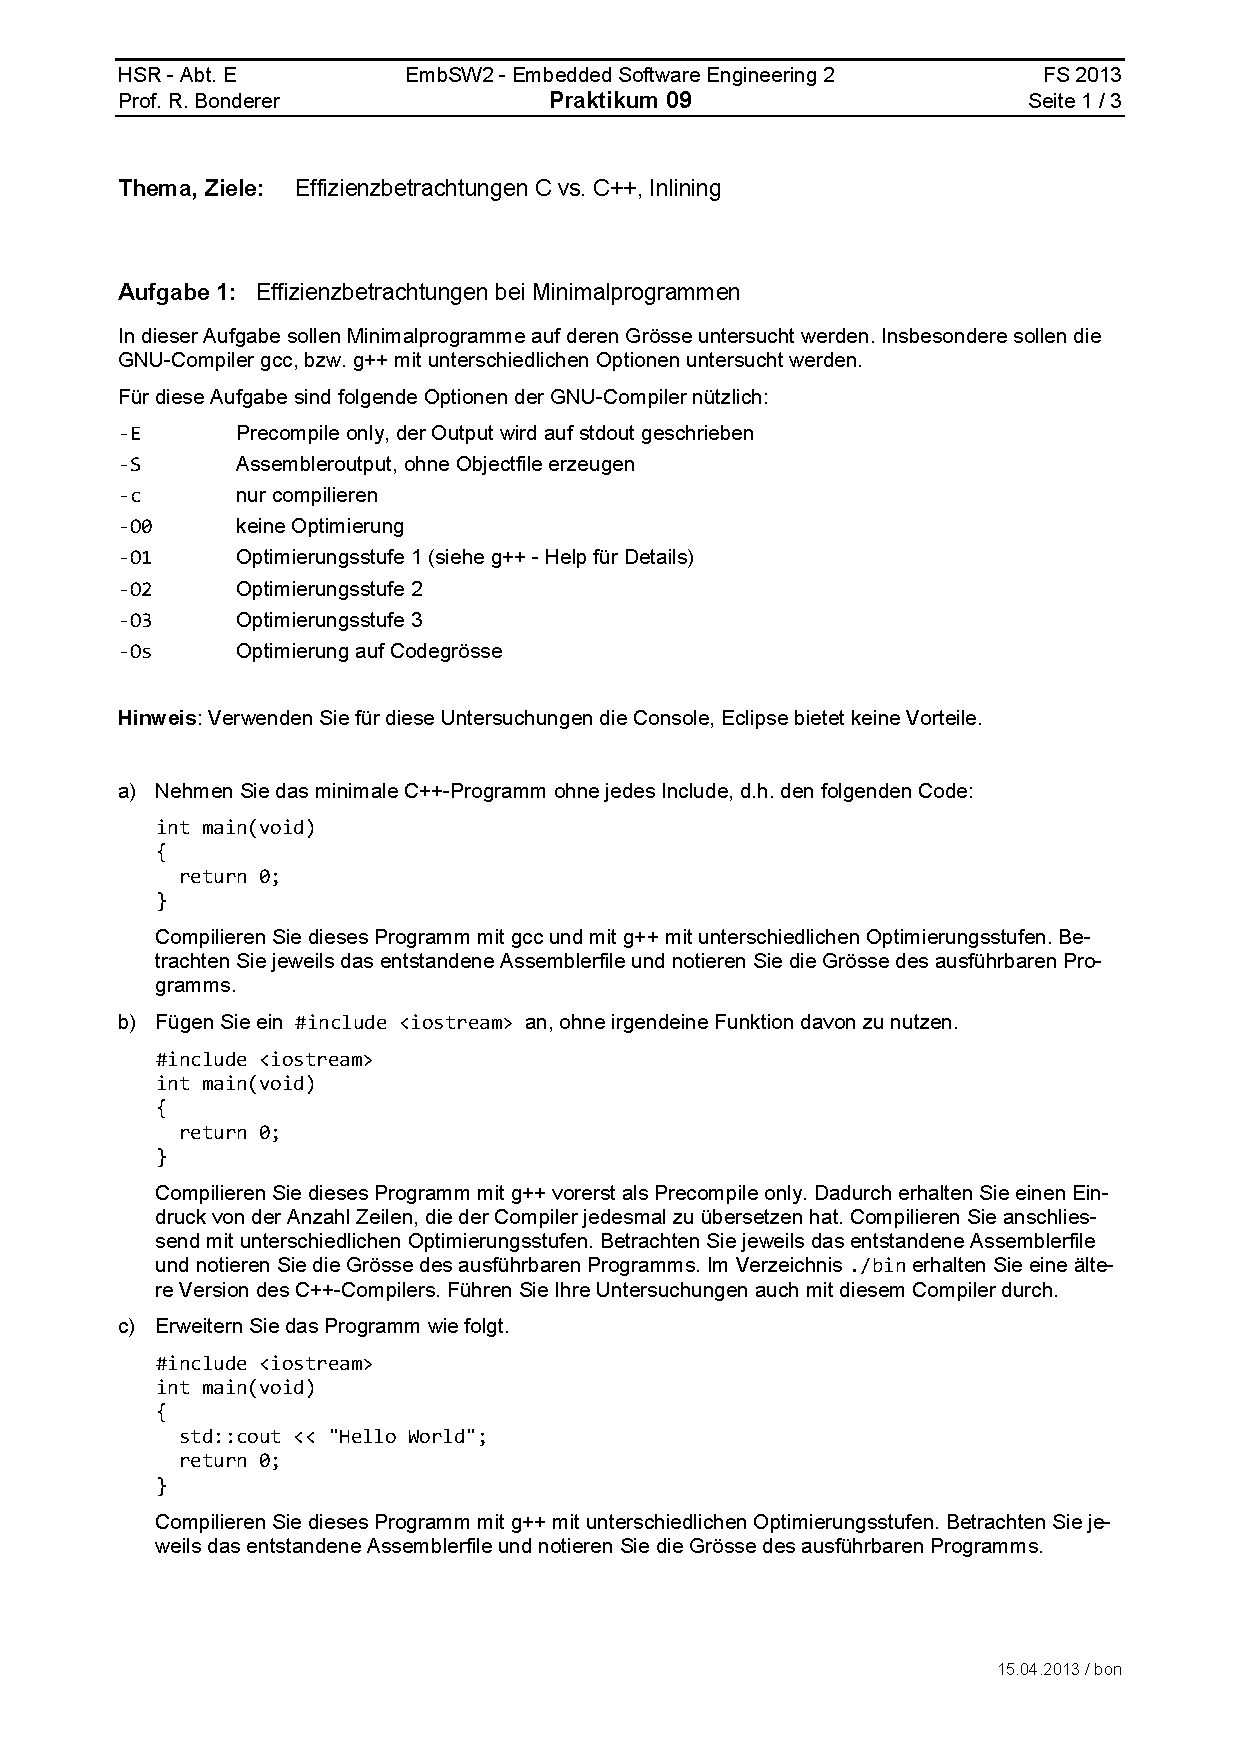
\includepdf[pages=-]{\basepath prak09/prak09.pdf}
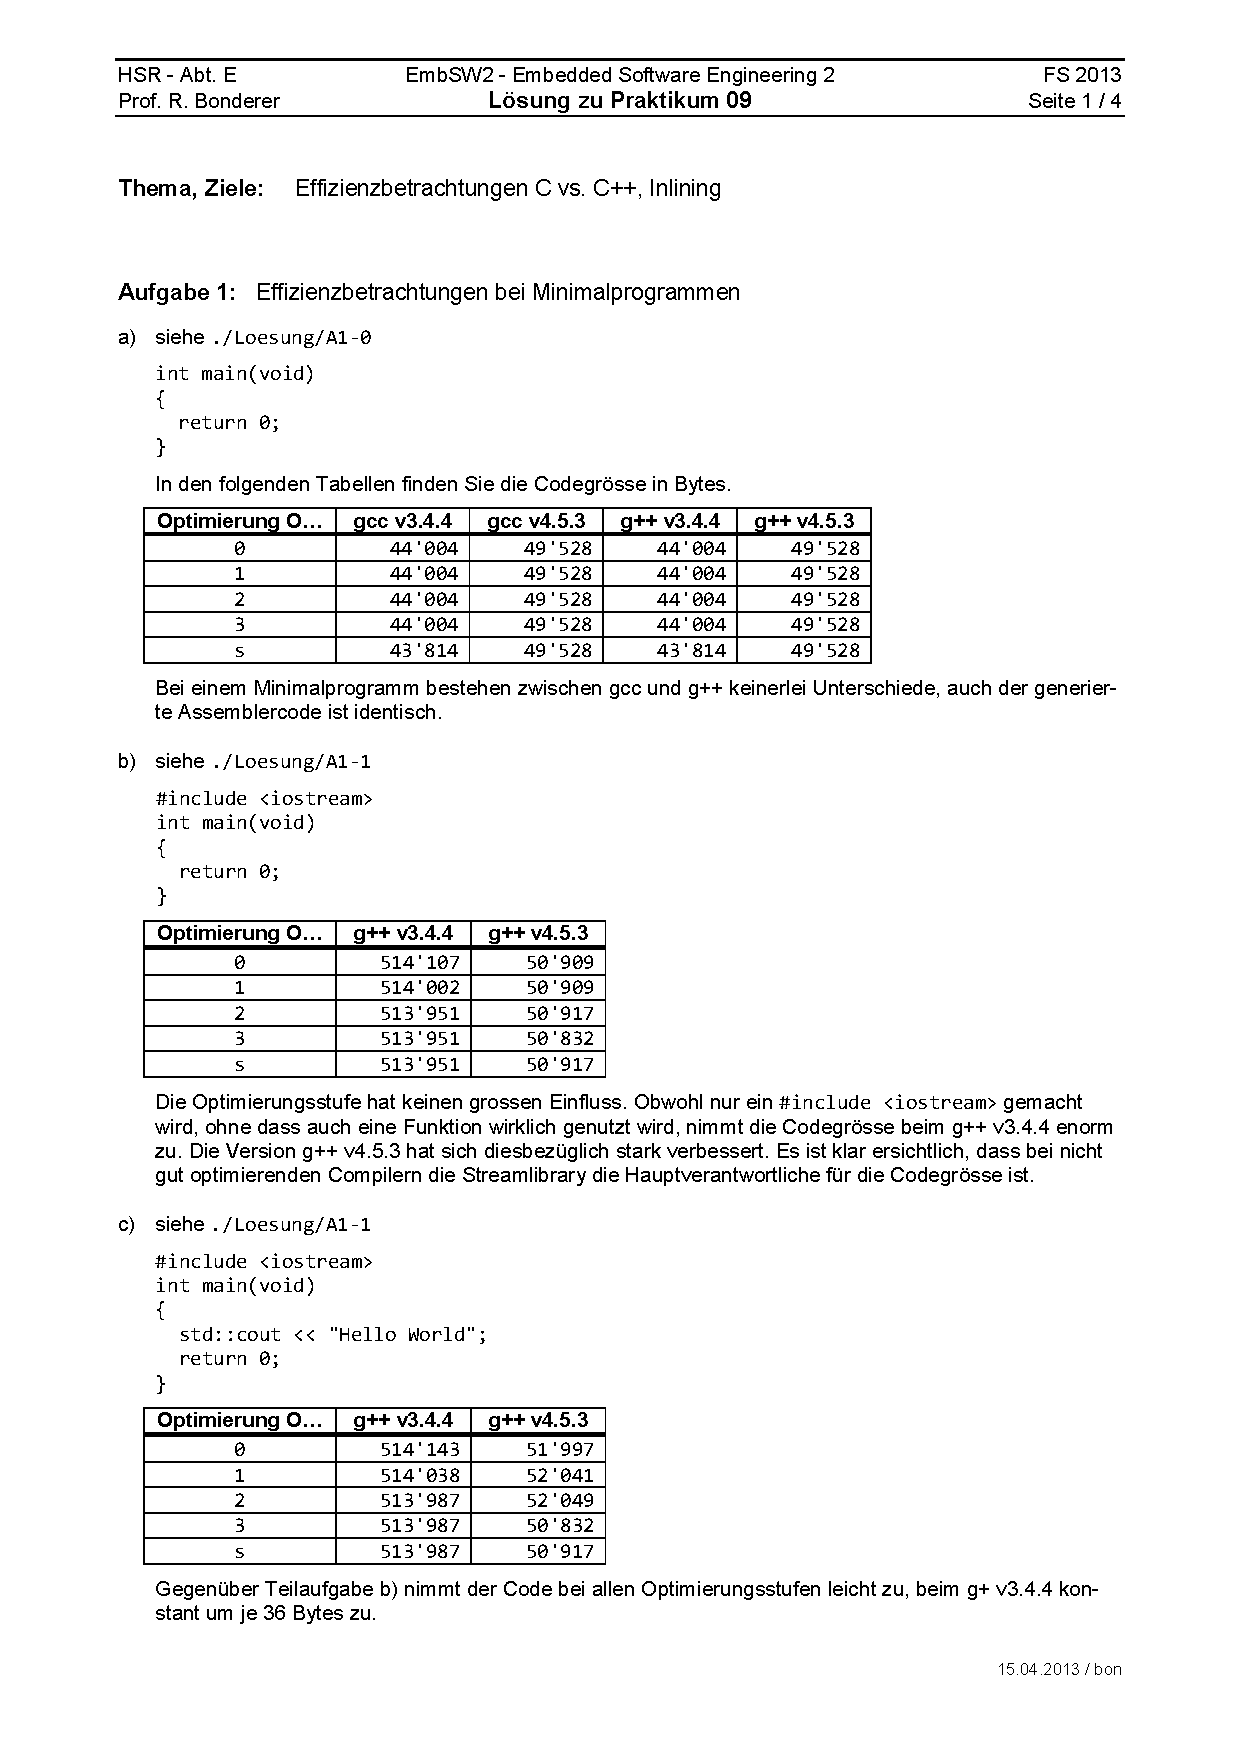
\includepdf[pages=-]{\basepath prak09/loesung09.pdf}
\section{Praktikum 9 Lösungen}
\lstinputlisting{\basepath prak09/Loesung/A1-0/main.cpp}
\lstinputlisting{\basepath prak09/Loesung/A1-1/main.cpp}
\lstinputlisting{\basepath prak09/Loesung/A1-2/main.cpp}
\lstinputlisting{\basepath prak09/Loesung/A2-1/main.cpp}
\lstinputlisting{\basepath prak09/Loesung/A2-1/rectangle.h}
\lstinputlisting{\basepath prak09/Loesung/A2-1/rectangle.cpp}
\lstinputlisting{\basepath prak09/Loesung/A2-2/main.cpp}
\lstinputlisting{\basepath prak09/Loesung/A2-2/rectangle.h}
\lstinputlisting{\basepath prak09/Loesung/A2-2/rectangle.cpp}
\lstinputlisting{\basepath prak09/Loesung/A2-3/main.cpp}
\lstinputlisting{\basepath prak09/Loesung/A2-3/rectangle.h}
\lstinputlisting{\basepath prak09/Loesung/A2-4/main.cpp}
\lstinputlisting{\basepath prak09/Loesung/A2-4/rectangle.h}
\lstinputlisting{\basepath prak09/Loesung/A2-5/main.cpp}
\lstinputlisting{\basepath prak09/Loesung/A2-5/rectangle.h}
\lstinputlisting{\basepath prak09/Loesung/A2-5/rectangle.cpp}

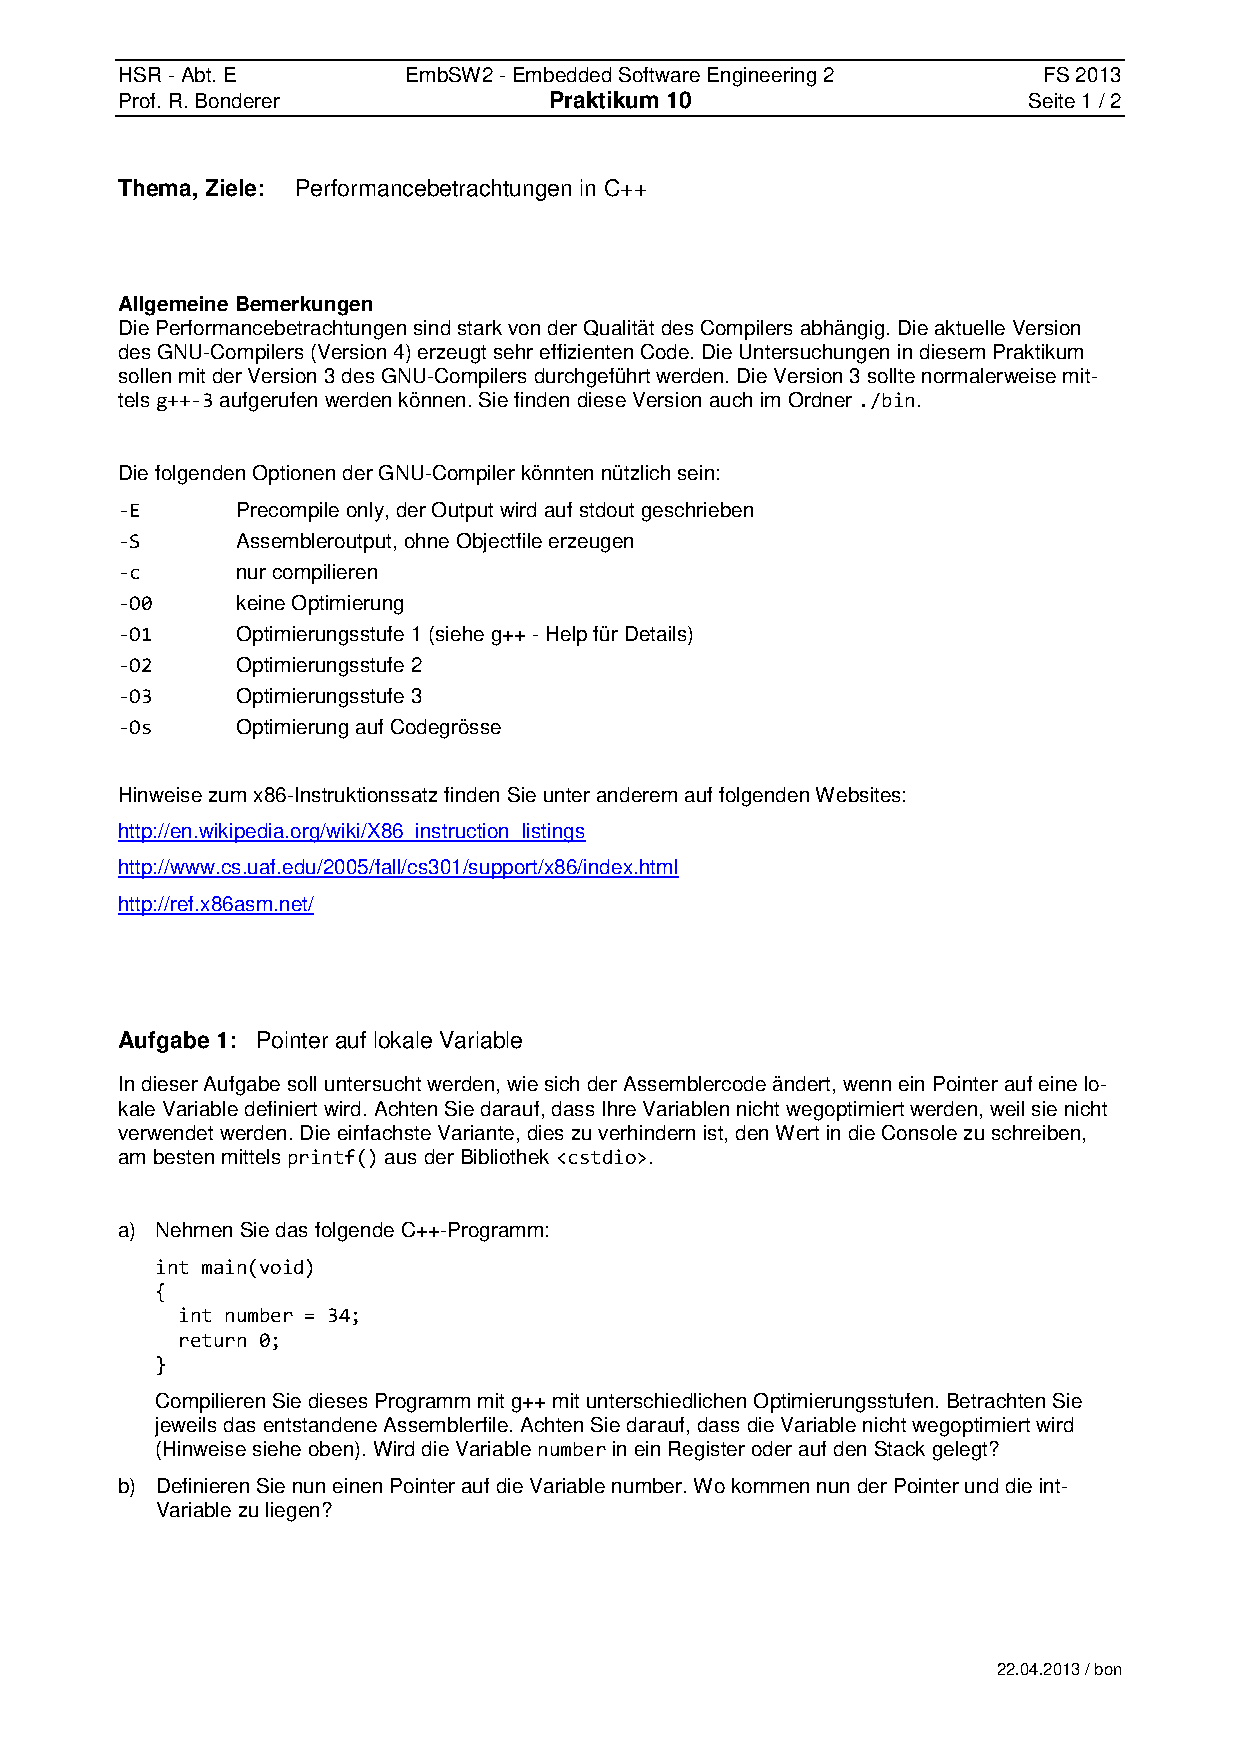
\includepdf[pages=-]{\basepath prak10/prak10.pdf}
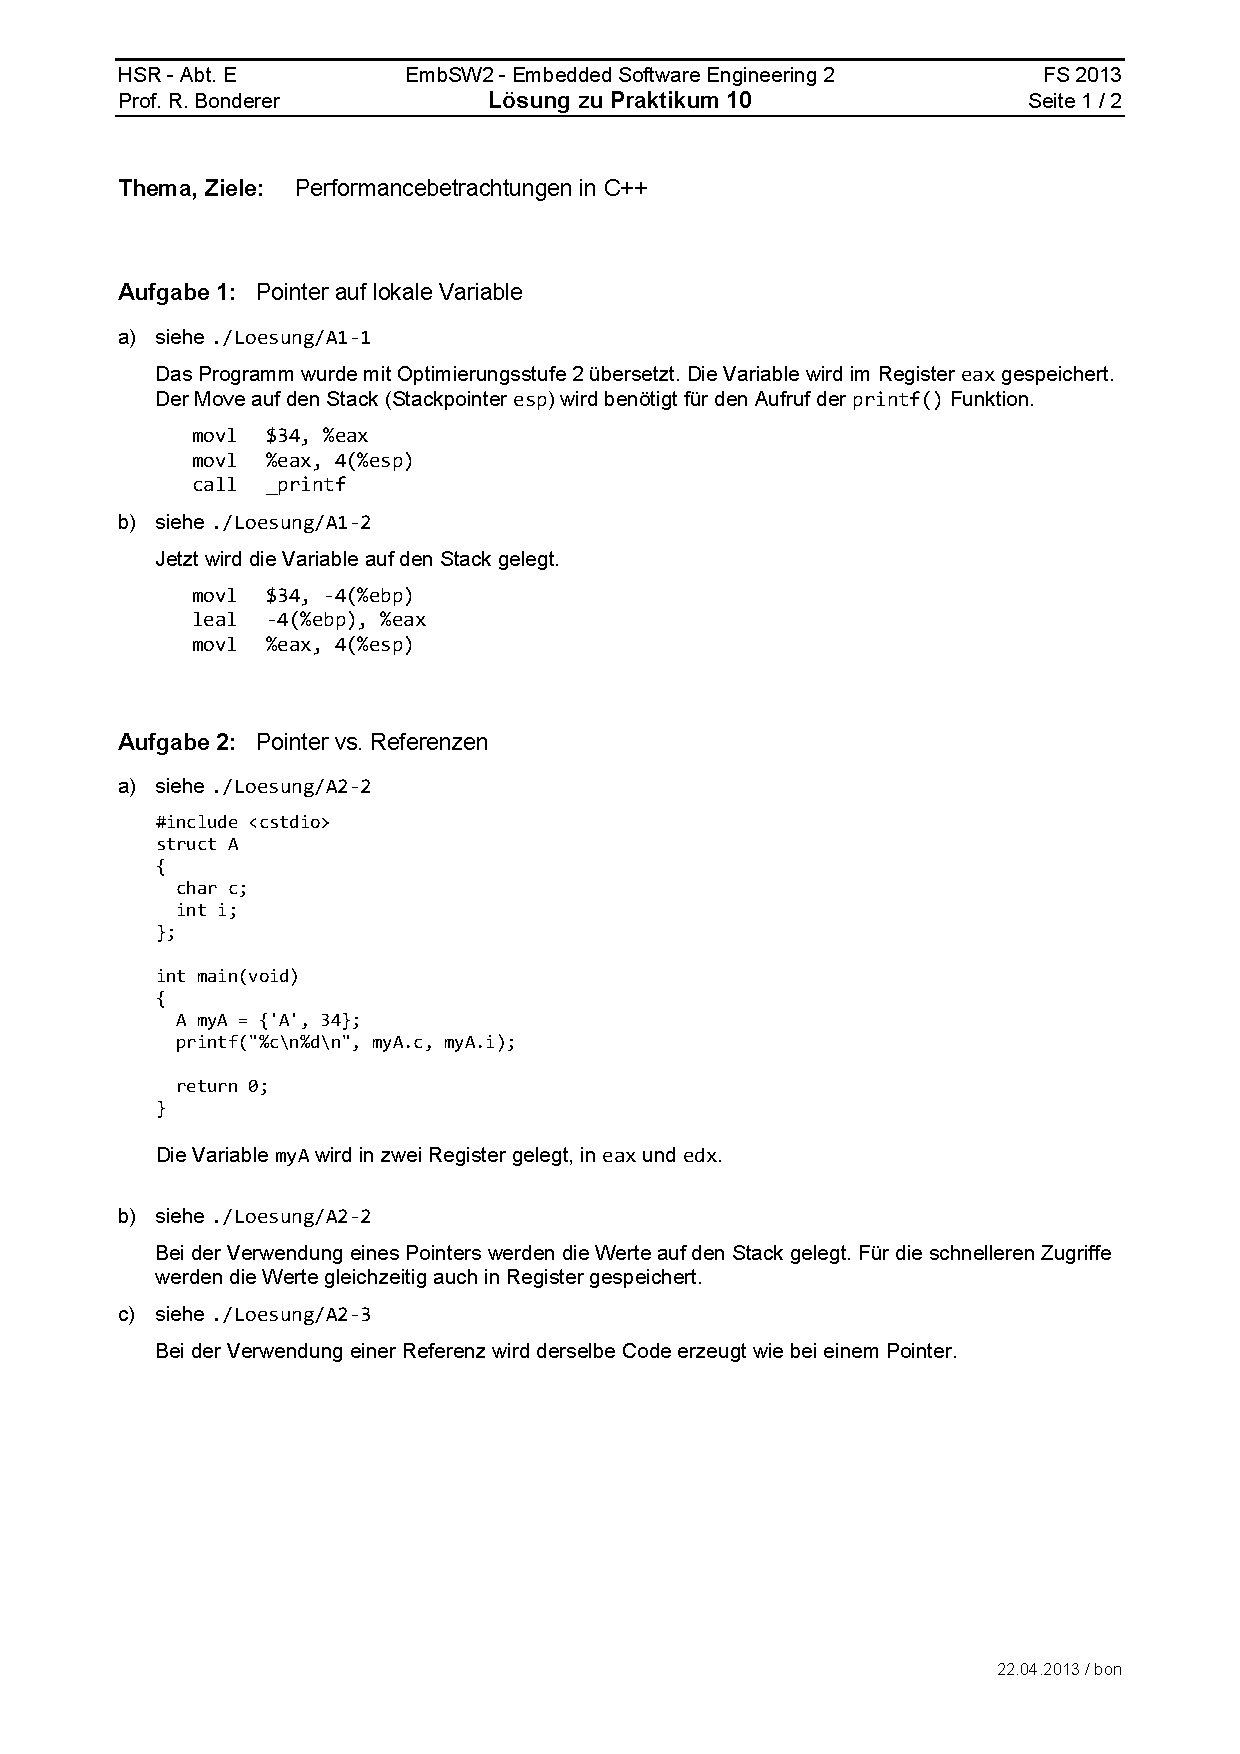
\includepdf[pages=-]{\basepath prak10/loesung10.pdf}
\section{Praktikum 10 Lösungen}
\lstinputlisting{\basepath prak10/Loesung/A1-1/main.cpp}
\lstinputlisting{\basepath prak10/Loesung/A1-2/main.cpp}
\lstinputlisting{\basepath prak10/Loesung/A2-1/main.cpp}
\lstinputlisting{\basepath prak10/Loesung/A2-2/main.cpp}
\lstinputlisting{\basepath prak10/Loesung/A2-3/main.cpp}
\lstinputlisting{\basepath prak10/Loesung/A3/main.cpp}
\lstinputlisting{\basepath prak10/Loesung/A4/main.cpp}

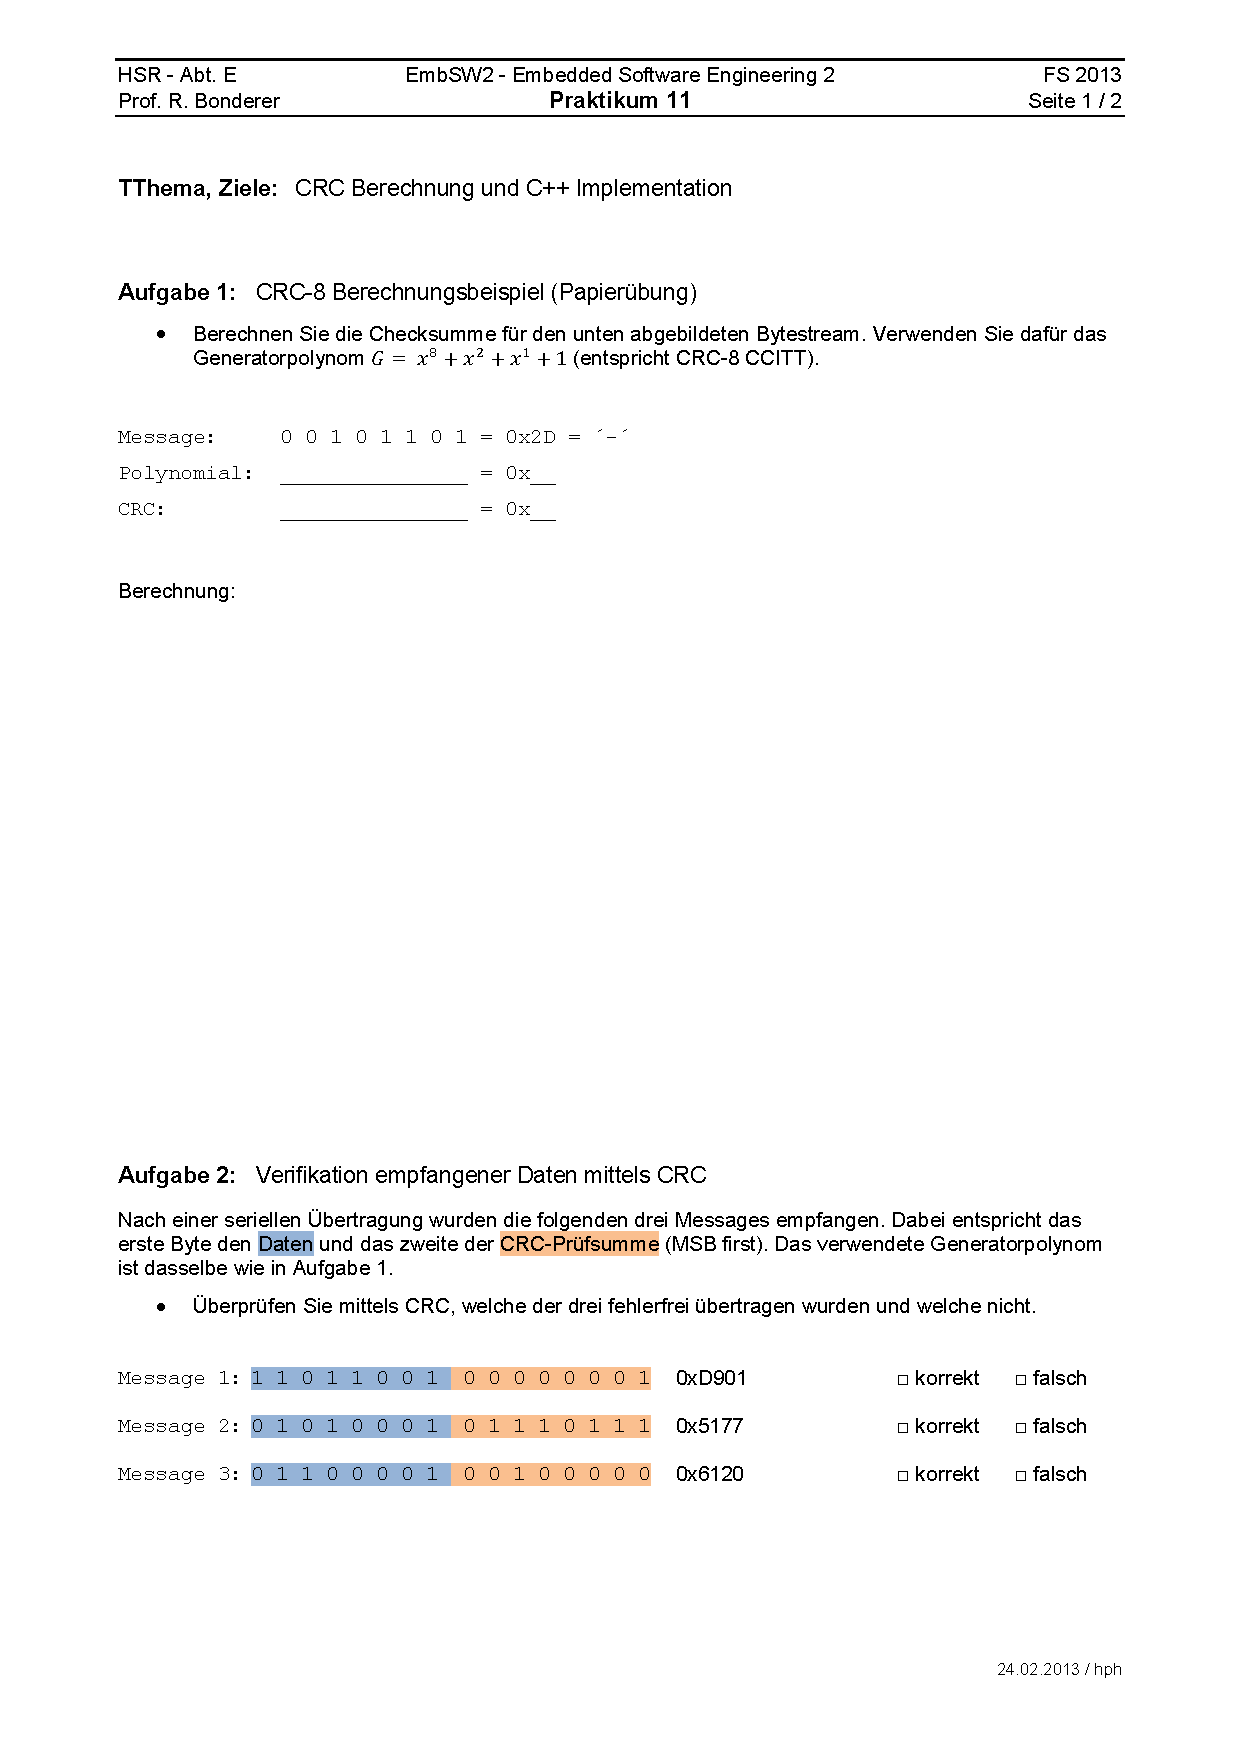
\includepdf[pages=-]{\basepath prak11/prak11.pdf}
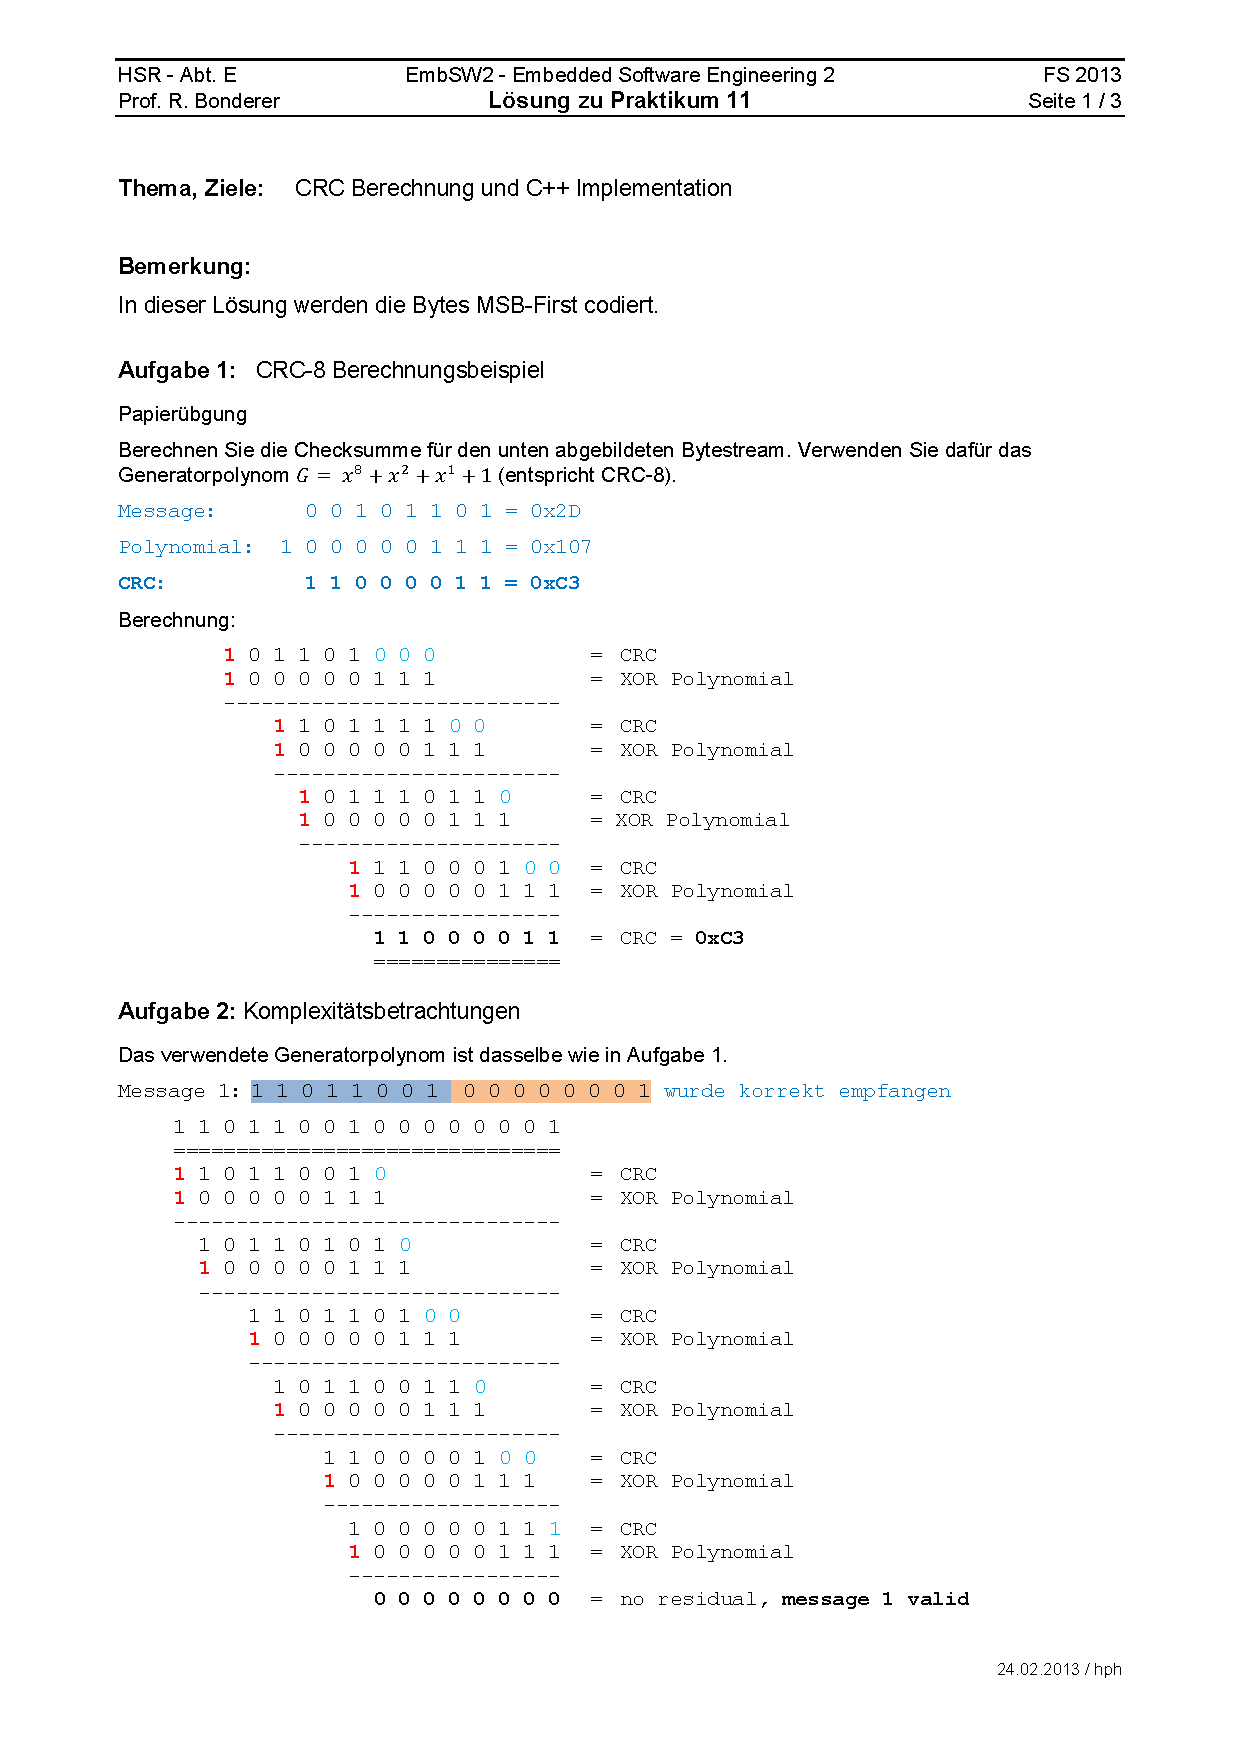
\includepdf[pages=-]{\basepath prak11/loesung11.pdf}
\section{Praktikum 11 Lösungen}
\lstinputlisting{\basepath prak11/Loesung/A3/crcTest.cpp}
\lstinputlisting{\basepath prak11/Loesung/A3/crc.h}
\lstinputlisting{\basepath prak11/Loesung/A3/crc.cpp}
\lstinputlisting{\basepath prak11/Loesung/A4/crcTest.cpp}
\lstinputlisting{\basepath prak11/Loesung/A4/crc.h}
\lstinputlisting{\basepath prak11/Loesung/A4/crc.cpp}

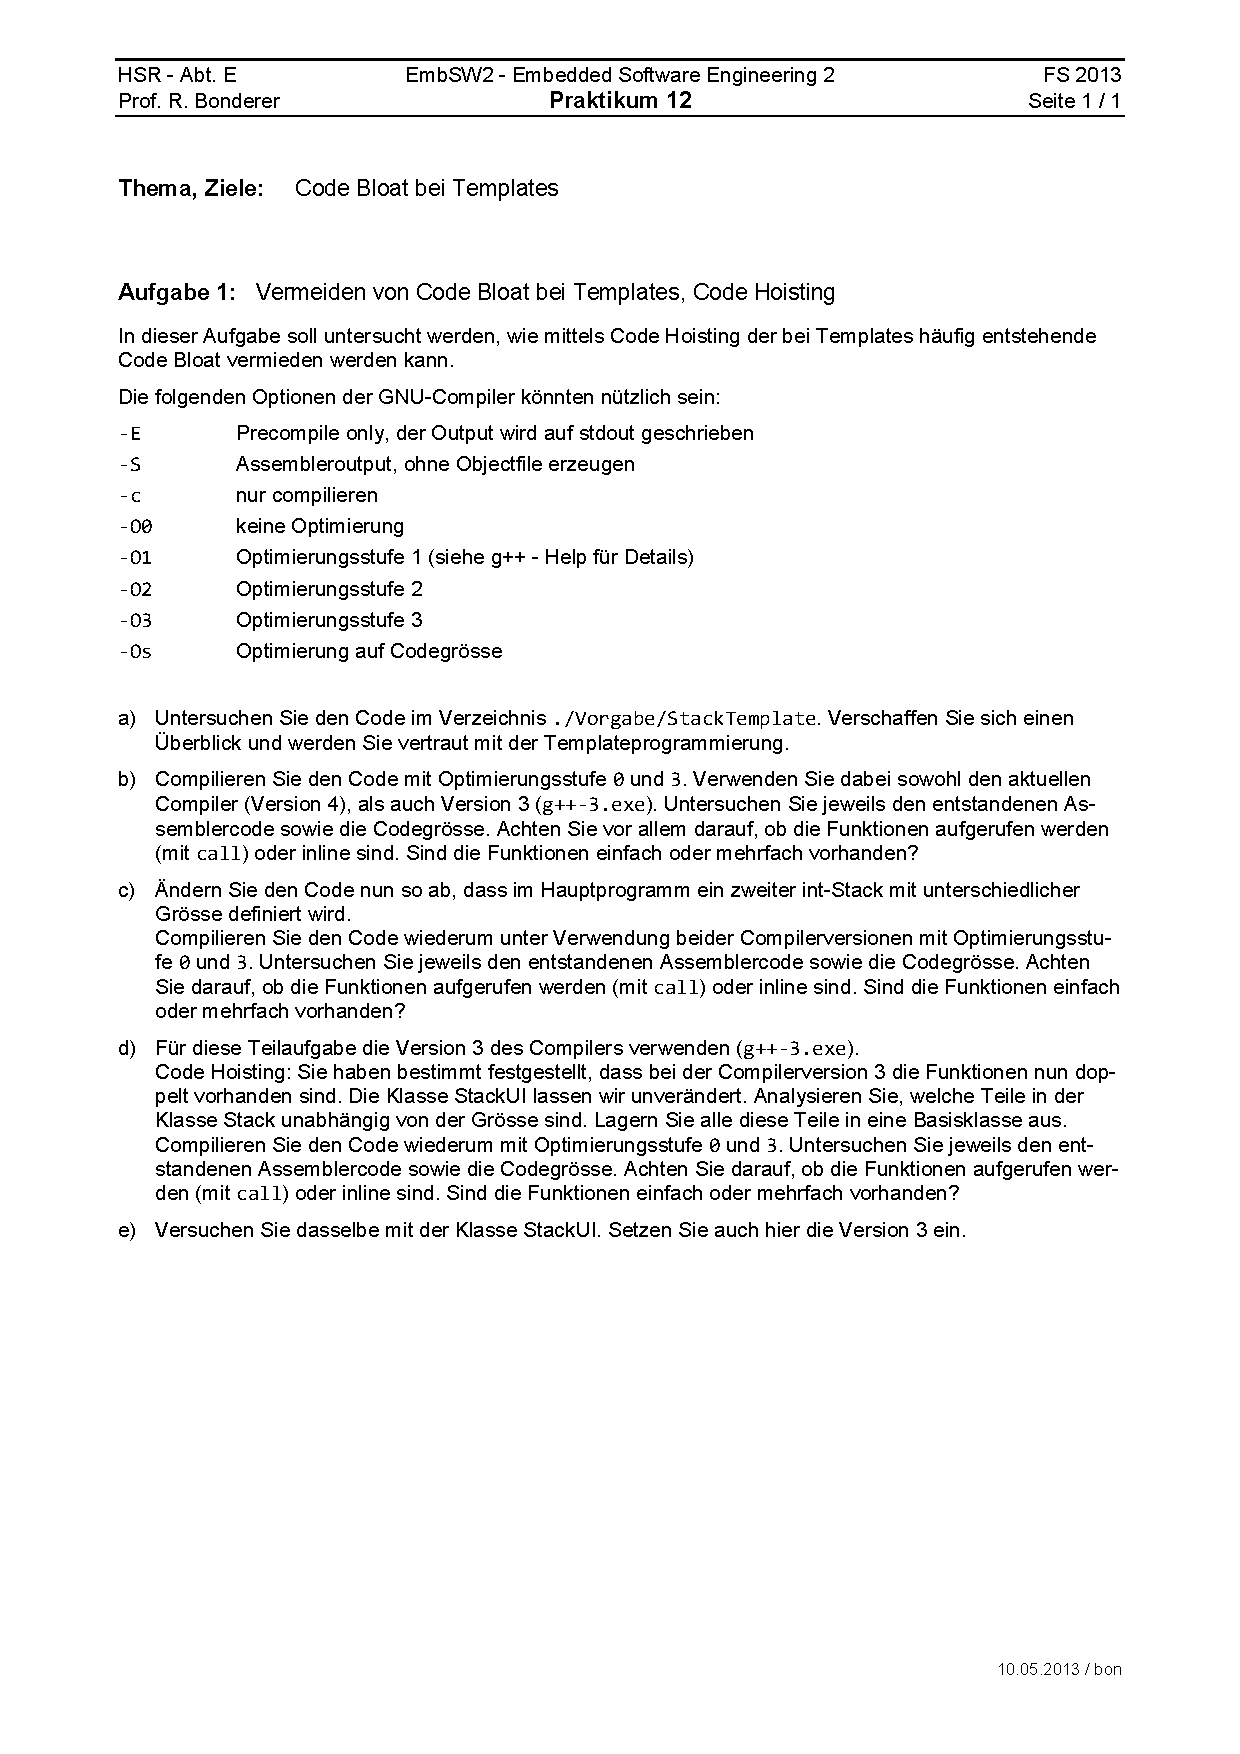
\includepdf[pages=-]{\basepath prak12/prak12.pdf}
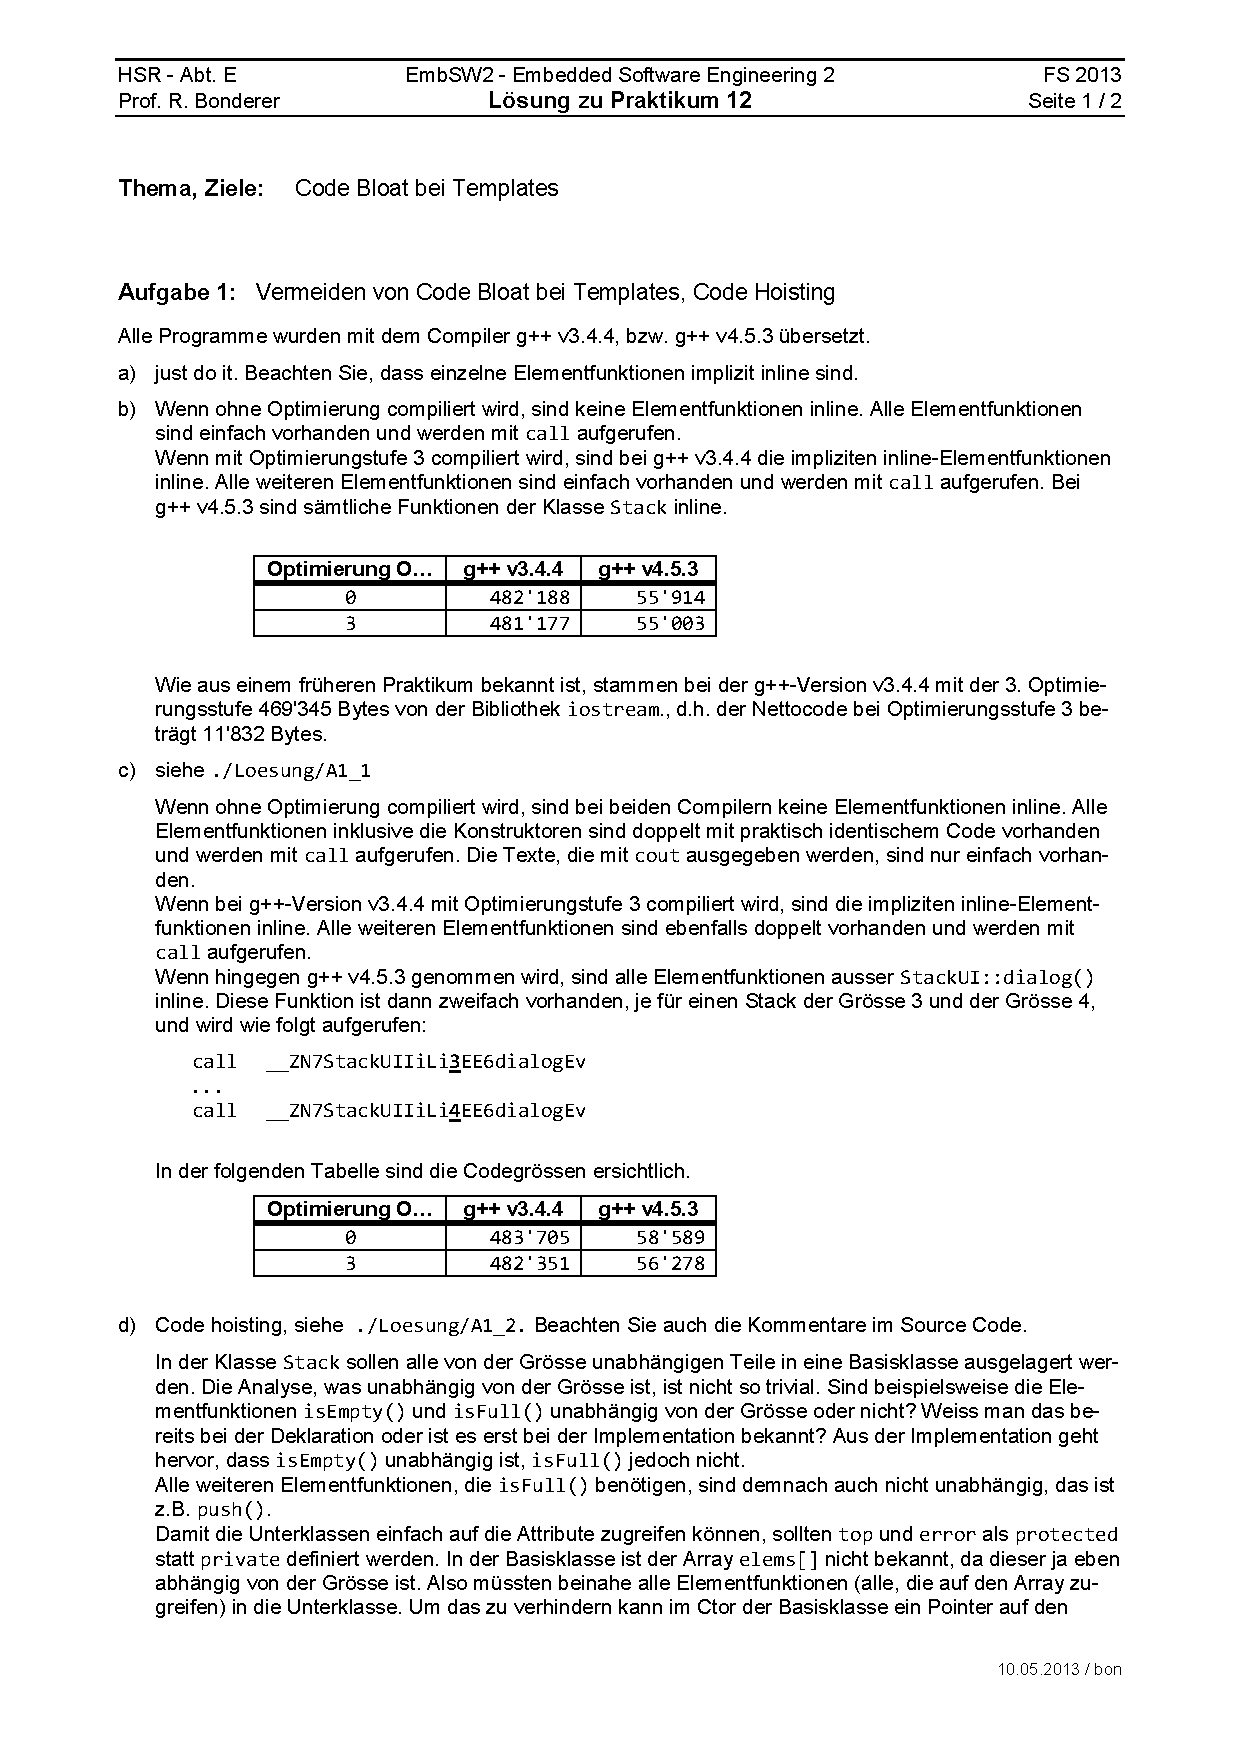
\includepdf[pages=-]{\basepath prak12/loesung12.pdf}
\section{Praktikum 12 Lösungen}
\lstinputlisting{\basepath prak12/Loesung/A1_1/stacktest.cpp}
\lstinputlisting{\basepath prak12/Loesung/A1_1/stack.h}
\lstinputlisting{\basepath prak12/Loesung/A1_1/stack.cpp}
\lstinputlisting{\basepath prak12/Loesung/A1_1/StackUI.h}
\lstinputlisting{\basepath prak12/Loesung/A1_1/StackUI.cpp}
\lstinputlisting{\basepath prak12/Loesung/A1_2/stacktest.cpp}
\lstinputlisting{\basepath prak12/Loesung/A1_2/stackNoSize.h}
\lstinputlisting{\basepath prak12/Loesung/A1_2/stackNoSize.cpp}
\lstinputlisting{\basepath prak12/Loesung/A1_2/stack.h}
\lstinputlisting{\basepath prak12/Loesung/A1_2/stack.cpp}
\lstinputlisting{\basepath prak12/Loesung/A1_2/StackUI.h}
\lstinputlisting{\basepath prak12/Loesung/A1_2/StackUI.cpp}

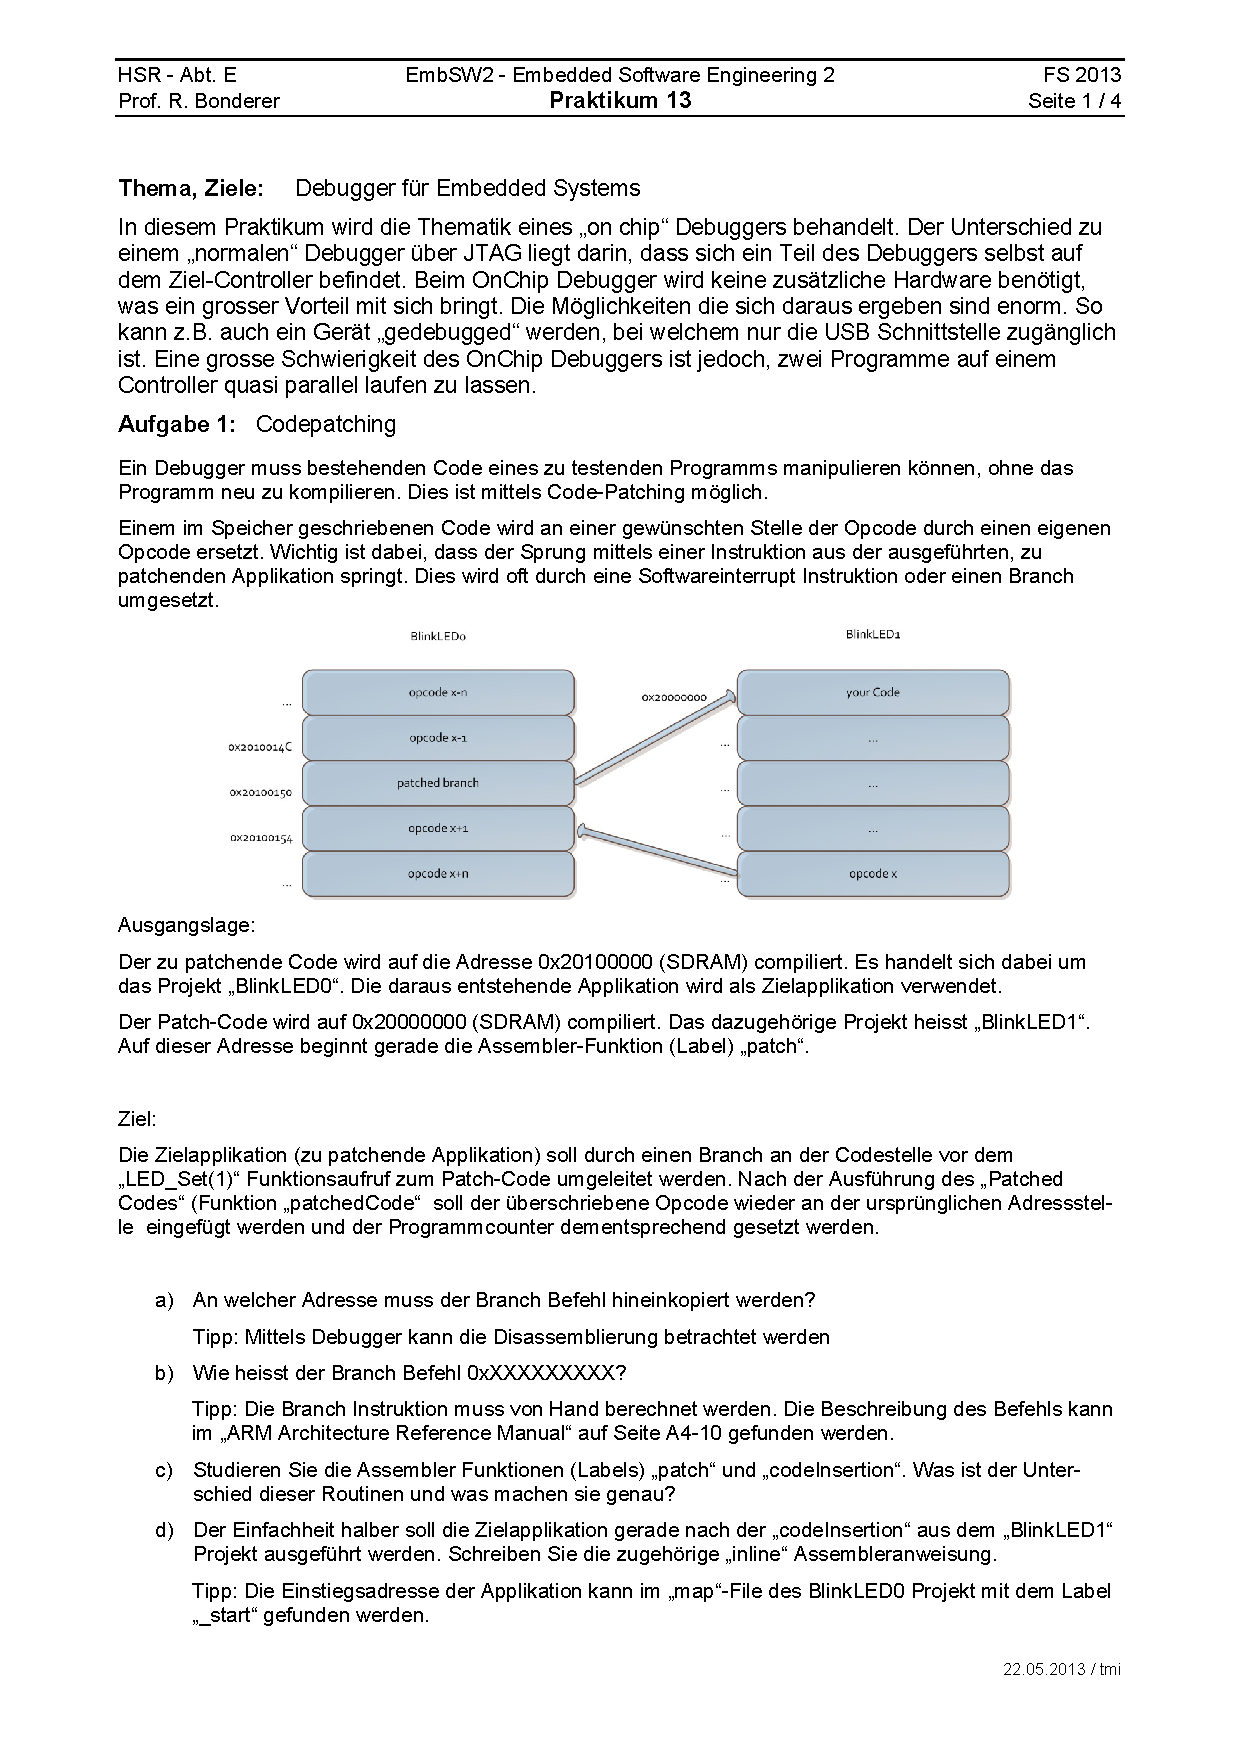
\includepdf[pages=-]{\basepath prak13/prak13.pdf}
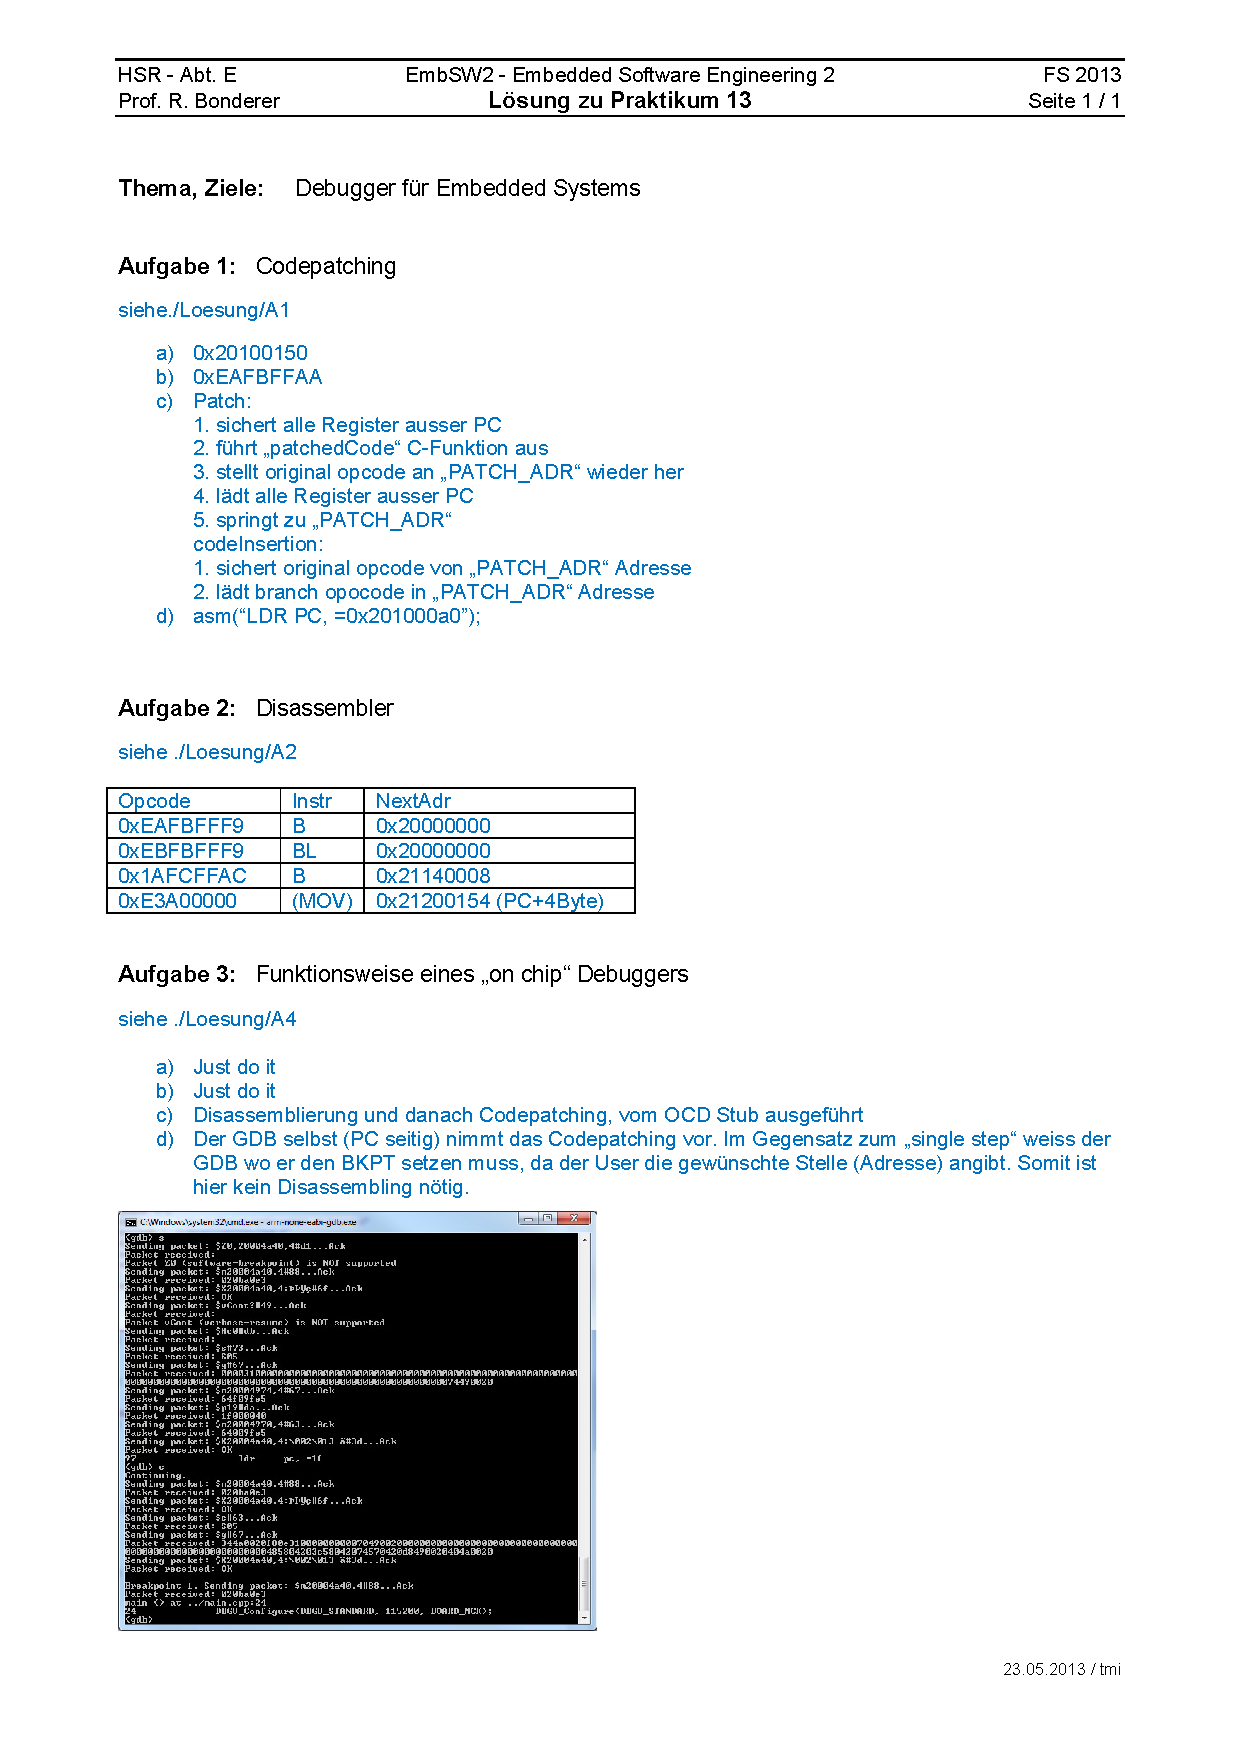
\includepdf[pages=-]{\basepath prak13/loesung13.pdf}
\section{Praktikum 13 Lösungen}
\lstinputlisting{\basepath prak13/Loesung/A1/BlinkLED0/main.cpp}
\lstinputlisting{\basepath prak13/Loesung/A1/BlinkLED1/main.cpp}
\lstinputlisting{\basepath prak13/Loesung/A2/ARMDisAsm/src/ARMDisAsmTest.cpp}
\lstinputlisting{\basepath prak13/Loesung/A2/ARMDisAsm/src/ARMDisAsm.h}
\lstinputlisting{\basepath prak13/Loesung/A2/ARMDisAsm/src/ARMDisAsm.cpp}
\lstinputlisting{\basepath prak13/Loesung/A2/ARMDisAsm/src/ARMReg.h}
\lstinputlisting{\basepath prak13/Loesung/A2/ARMDisAsm/src/ARMReg.cpp}


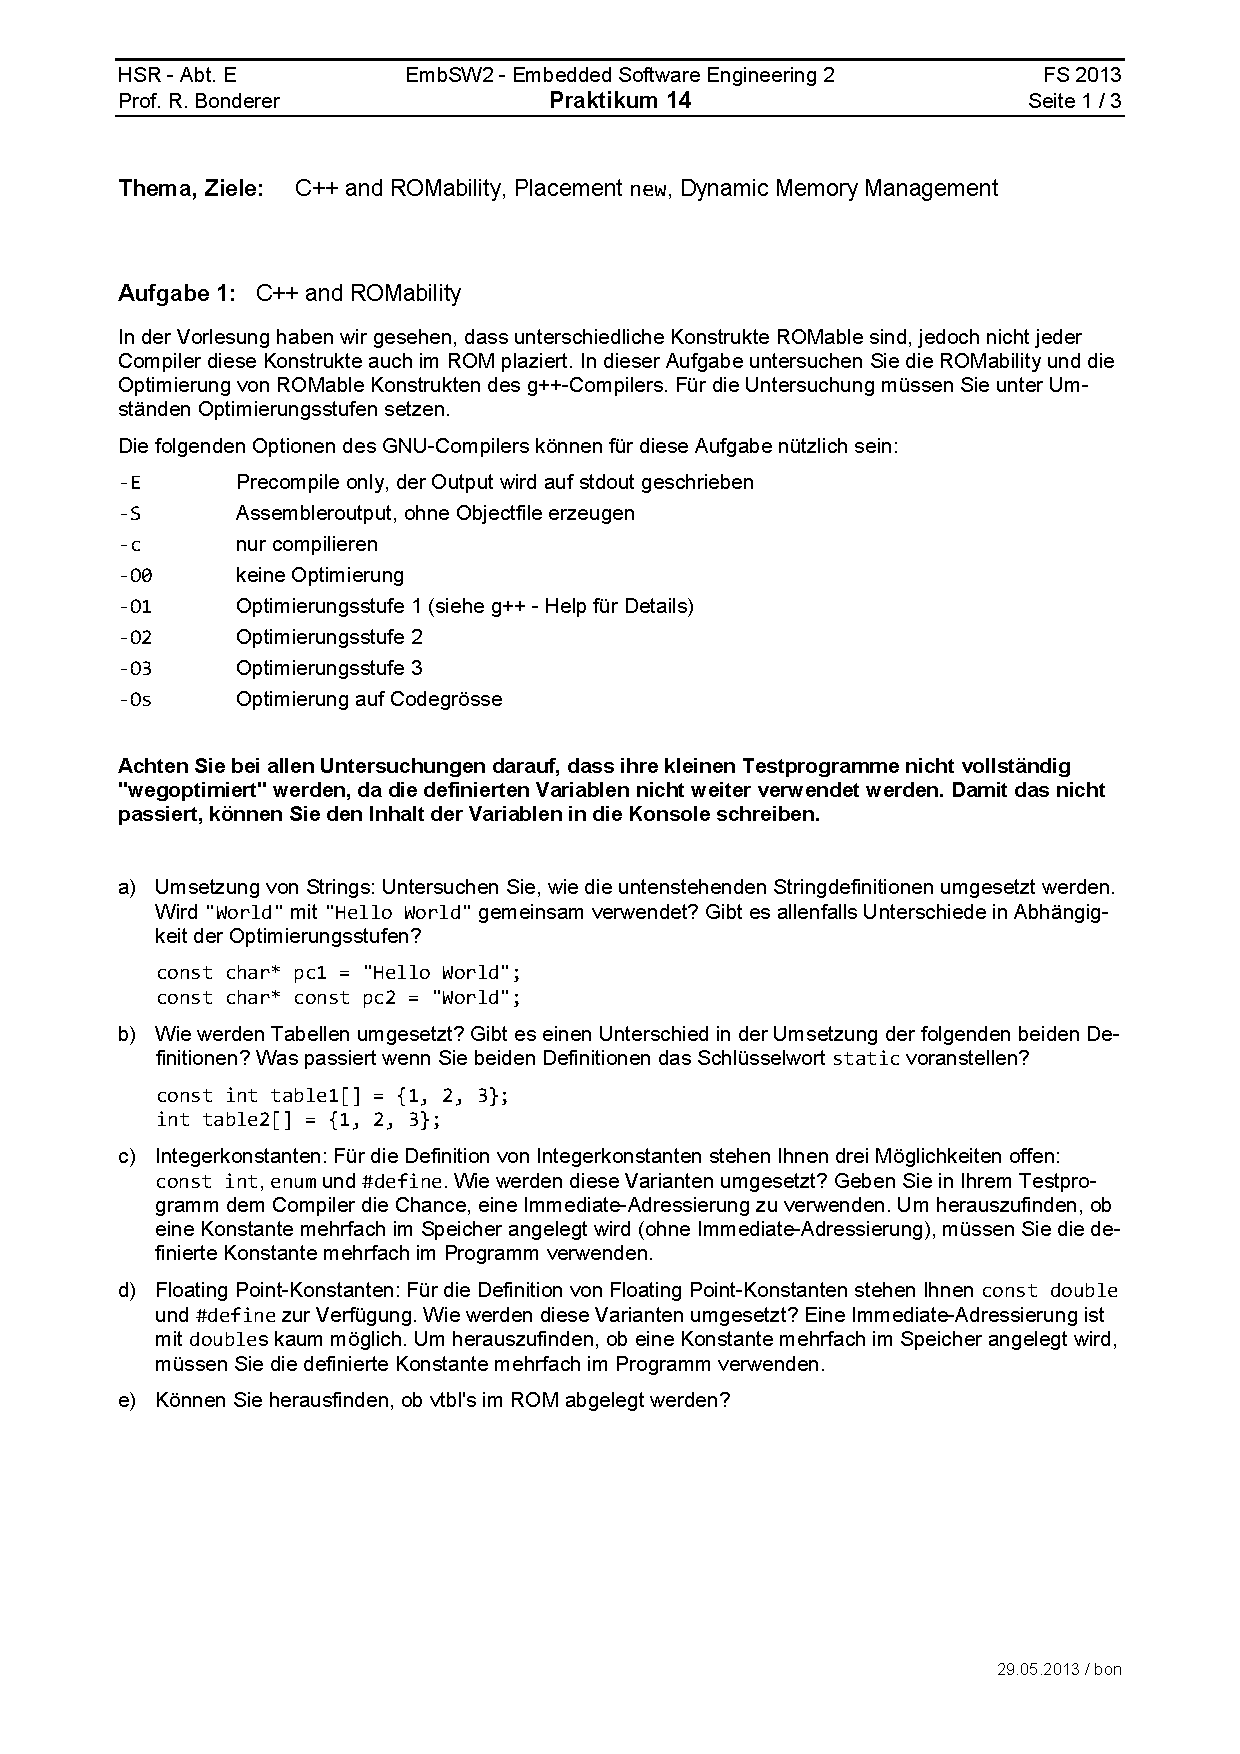
\includepdf[pages=-]{\basepath prak14/prak14.pdf}
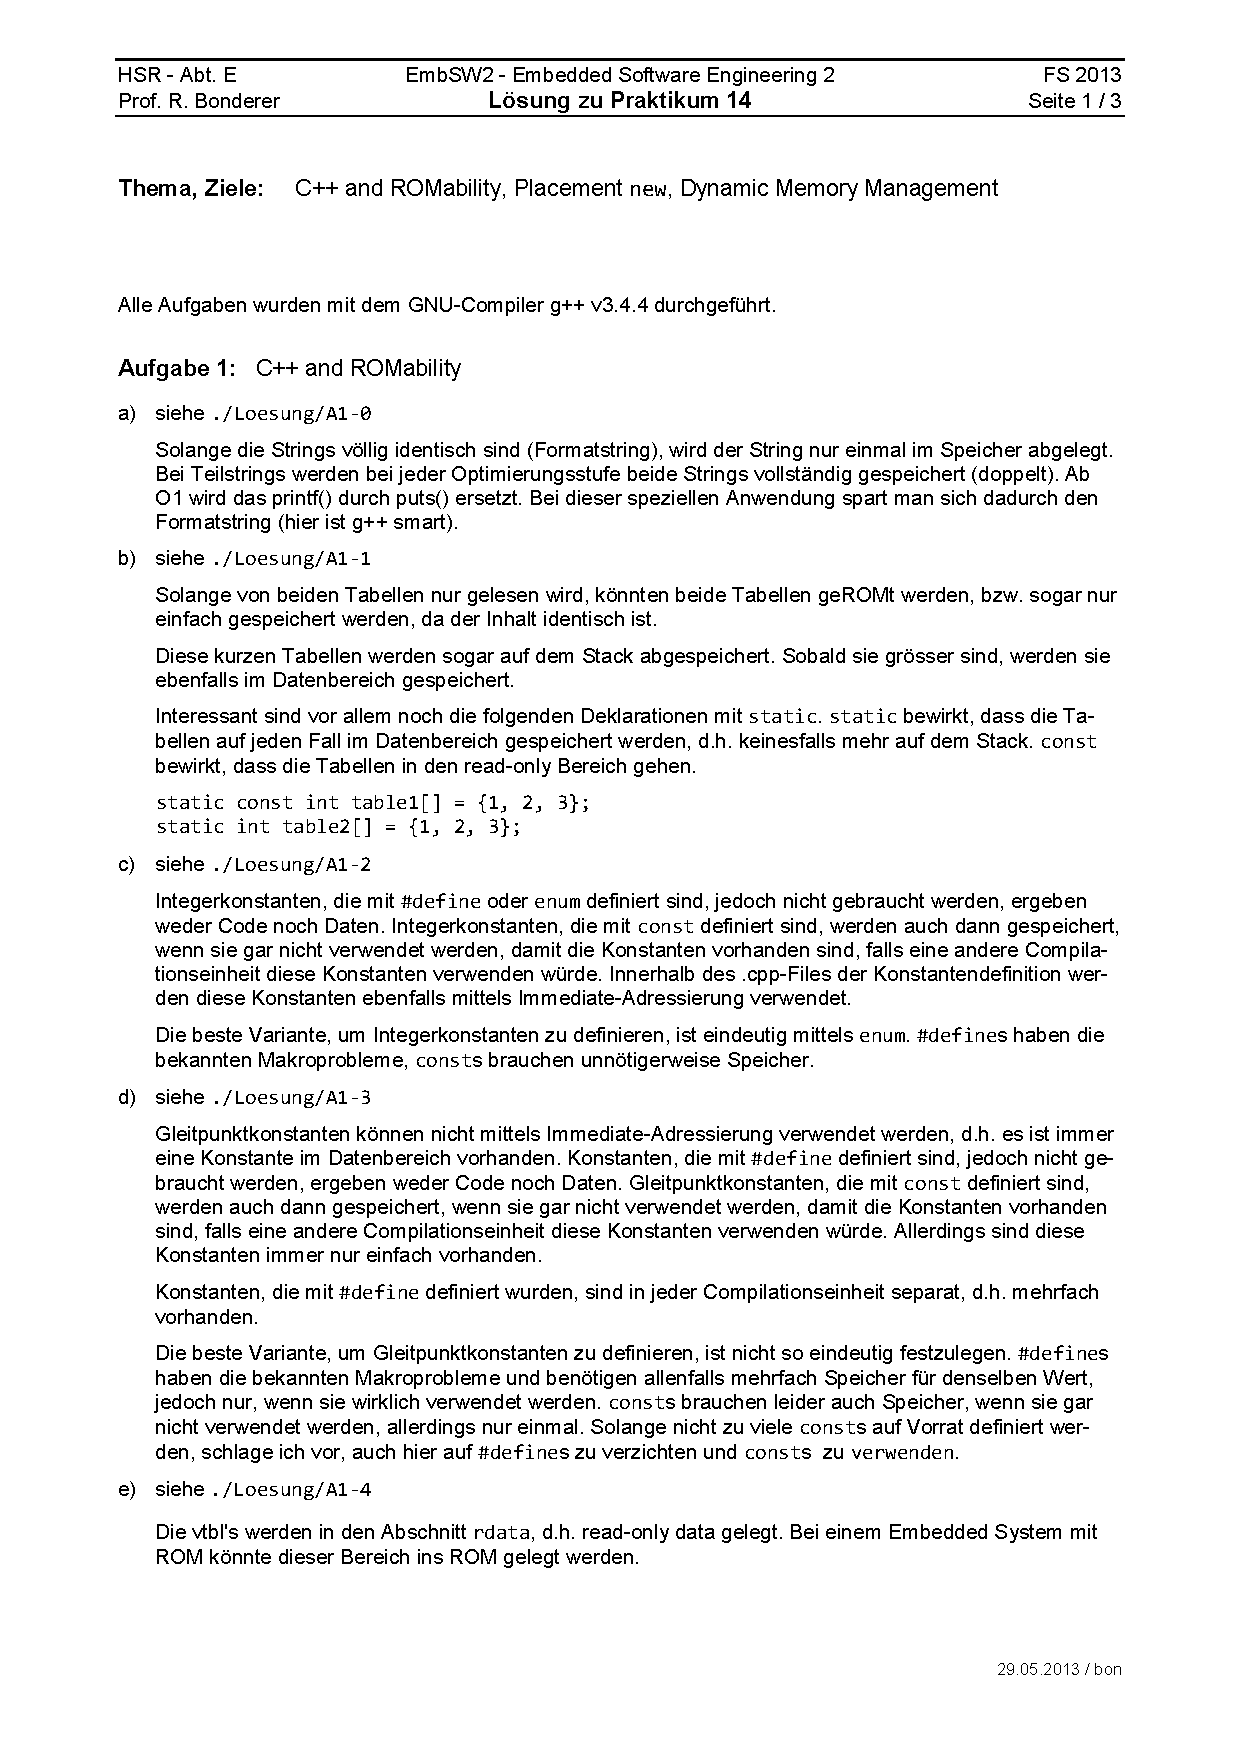
\includepdf[pages=-]{\basepath prak14/loesung14.pdf}
\section{Praktikum 14 Lösungen}
\lstinputlisting{\basepath prak14/Loesung/A1-0/main.cpp}
\lstinputlisting{\basepath prak14/Loesung/A1-1/main.cpp}
\lstinputlisting{\basepath prak14/Loesung/A1-2/main.cpp}
\lstinputlisting{\basepath prak14/Loesung/A1-2/ints.h}
\lstinputlisting{\basepath prak14/Loesung/A1-2/subs.cpp}
\lstinputlisting{\basepath prak14/Loesung/A1-3/main.cpp}
\lstinputlisting{\basepath prak14/Loesung/A1-3/floats.h}
\lstinputlisting{\basepath prak14/Loesung/A1-3/subs.cpp}
\lstinputlisting{\basepath prak14/Loesung/A1-4/main.cpp}
\lstinputlisting{\basepath prak14/Loesung/Placement/placement.cpp}
\lstinputlisting{\basepath prak14/Loesung/FixedPool/src/FixedPool.cpp}
\lstinputlisting{\basepath prak14/Loesung/FixedPool/src/PoolAllocator.h}
\lstinputlisting{\basepath prak14/Loesung/FixedPoolCeil/src/FixedPoolCeil.cpp}
\lstinputlisting{\basepath prak14/Loesung/FixedPoolCeil/src/PoolAllocator.h}
\lstinputlisting{\basepath prak14/Loesung/BlockAllocation/src/BlockAllocation.cpp}
\lstinputlisting{\basepath prak14/Loesung/BlockAllocation/src/BlockAllocator.h}
\lstinputlisting{\basepath prak14/Loesung/BlockAllocation/src/PoolAllocator.h}
\end{document}
